\RequirePackage{docswitch}
\setjournal{\flag}

\documentclass[twocolumn]{aastex62}
% Custom commands from LSST DESC, see texmf/styles/lsstdesc_macros.sty
\usepackage{lsstdesc_macros}
\usepackage{tikz}
\usetikzlibrary{calc}
\usepackage{mwe}
\usepackage[htt]{hyphenat}
\usepackage{graphicx}
\graphicspath{{./}{./figures/}}
\bibliographystyle{aj}
\extrafloats{100}
\usepackage{hyperref}
% Add your own macros here:
\newcommand{\rachel}[1]{{\textcolor{cyan}{{\textbf (RM: #1)}}}}
\newcommand{\as}[1]{{\textcolor{magenta}{{\textbf (AS: #1)}}}}


%
% ======================================================================

\begin{document}

\title[LSST DESC DC1]{The LSST DESC Data Challenge 1: Generation and Analysis of Synthetic Images for Next Generation Surveys }

%\maketitlepre

\begin{abstract}

The success of the Large Synoptic Survey Telescope (LSST) as a dark energy experiment will depend on controlling systematic biases in cosmological probes. Simulations are critical for developing the methodology to estimate and mitigate these systematics. In the first Data Challenge from the LSST Dark Energy Science Collaboration, we evaluate potential systematic biases in observables, with an emphasis on galaxy clustering. We simulate LSST images, then process and analyze them using the \as{development} version of the LSST Data Management pipeline. Then we characterize the resulting systematics and implement corrections. We also analyze different dithering strategies and check their impact mitigating potential systematic effects. Our results demonstrate that we can generate realistic LSST-like simulated images and control the systematic effects, after processing these images, at a sufficient level to enable major advances in our knowledge of dark energy and cosmology. The methodology presented here can be easily translated to current and future imaging surveys.
\as{I'm not sure I like this abstract. It depends how exactly you want to spin it, but I would stress more the 'lessons learned' aspect of DC1}

\end{abstract}

% Keywords are ignored in the LSST DESC Note style:
\dockeys{large-scale structure of the universe}

\section{Introduction}
\label{sec:intro}
\as{Edited the section below a little.}
The increase in statistical power from recent cosmological experiments makes the modeling and mitigation of systematic uncertainties key to extracting the maximum amount of information from these surveys. More traditional in high energy particle physics~\citep{Brun:118715, 2006JHEP...05..026S}, end-to-end simulations provide a unique framework to
model systematics and streamline processing and analysis pipelines given out complete understanding of the inputs and outputs. With the increasing availability of computational resources, this approach has also been extended to imaging surveys~\citep{2016ApJ...817...25B}, and similar efforts are being undertaken in spectroscopic surveys such as DESI~\citep{2016arXiv161100036D}.

For surveys like the LSST~\citep{Overview}, where the expected data volume is very large, and where a highly stringent control of the systematic uncertainties is required, producing these
kind of end-to-end simulations enables successful validation and verification of the processing and
analysis pipelines. With a total of $\sim 50$ PB of raw data and $\sim 40$ billion objects~\citep{Overview} after 10 years, the
data handling becomes challenging even when considering a small subset of the LSST area.  

The LSST Dark Energy Science Collaboration
(DESC\footnote{\url{http://lsstdesc.org/}}) has planned a series of
Data Challenges (DCs) carried out over a period of years, aimed at
successively more stringent and comprehensive tests of analysis
pipelines, to ensure adequate control of systematic uncertainties for
analysis of the LSST data.  An additional goal of these DCs is
development of the infrastructure for analyzing, storing, and serving
substantial data volumes; even while using the outputs of the LSST
Data Management (DM) stack as inputs into analysis pipelines, the
analysis pipelines will need to handle quantities of data beyond those
seen by ongoing surveys, even after just a single year of LSST data is
available. Moreover, it is anticipated that non-negligible subsets of
the data may need to be reprocessed to generate systematic error
budgets (e.g., assessing sensitivity of the results to certain stages
of the analysis process by changing some parameters in the
analysis). These goals will be achieved in practice by a combination
of reprocessing of the precursor datasets, which have the advantage of
being realistic and completely synthethic datasets, which have the
advantage of both having a known ground truth and the ability to turn
various effects on and off and thus study them in a more controlled
environment.

Both goals of the DCs dictate a gradual increase in the
sophistication and volume of the simulated data In this paper, we
present and analyze simulated images from DC1, the first of three such
data challenges planned withing DESC. The nominal goal of this dataset
is to produce synthetic data corresponding to 10 years of integration
in the $r$-band over a contiguous patch of the sky covering approximately 40 deg$^{2}$ of the
sky. This represents just one of the LSST's six filters and covers a rather 
small fraction ($\sim$ 0.2\%) of the total LSST area. In this paper we
describe how this was achieved and  characterize the resulting
products. We validate the basic photometric and astromatric
calibration of these products and check the performance of the
pipeline against the requirements set by LSST and DESC in their
respective Science Requirements Documents~\citep{LPM-17,
  2018arXiv180901669T}. These data products encompass single-visit and
coadded calibrated exposures (i.e., flattened, background subtracted,
etc.) and source catalogs that take up to $\sim 225$ TB of disk
space. To check suitability of this dataset for galaxy clustering
measurements, we perform the two-point clustering analysis in harmonic space for these simulations and assess the impact of different observing conditions/foregrounds as potential sources of systematic effects and how dithering can mitigate them. 

This paper is structured as follows: \secref{design} includes a summary of the factors that informed
the design of this data challenge.  In \secref{inputs}, we describe the inputs for our simulated images. In \secref{dithering}, we discuss the dither strategies used for this study. In \secref{image_generation_pipeline}, we describe the process used to generate, process and reduce LSST-like artificial images. In \secref{catalogs}, we describe the processed data products generated and perform several validation tests. In \secref{data_selection} we describe the procedure to obtain a clean data sample suitable for clustering analyses. In \secref{results}, we present the clustering analyses on the simulated data products. Finally, in \secref{conclusions}, we present some concluding remarks.

\section{Data Challenge Design}
\label{sec:design}

As mentioned in \secref{intro}, the design of this first data challenge (DC1) is driven by a
combination of several factors: the need to test analysis pipelines for control of systematic
uncertainty, and to develop infrastructure for processing and serving data in a way that is useful
to DESC.  While the subsequent data challenges DC2 and DC3 are intended to be full-collaboration activities, DC1 is more limited in
scope and focus, with a goal of enabling tests of the large-scale structure (LSS) working group
pipelines for analysis and systematics mitigation of two-point clustering statistics.
\as{Come on, that is absolute bullshit. This was supposed to be a full
  collaboration activity, but it never turned out that way and as it
  was superseeded by DC2. No need to make LSS somehow responsible for
  DC1. :-) }
\begin{figure}
\centering
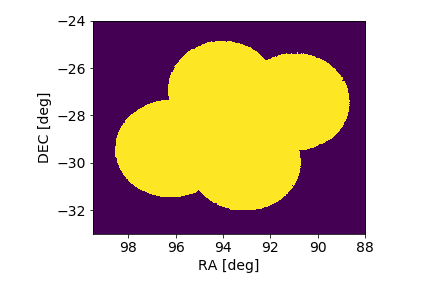
\includegraphics[width=0.9\columnwidth]{footprint.png}
\caption{Footprint of the DC1 dataset. We simulate 4 LSST full focal plane pointings which roughly corresponds to 40 deg$^{2}$.}
\label{fig:footprint}
\end{figure}

As a stepping stone to eventually producing images covering hundreds to thousands of square degreees
in DC2 and DC3, DC1 covers a $40$ deg$^2$ footprint.  This is sufficient to enable tests of
two-point clustering statistics up to $\sim 1$ degree scales.  To ensure the simulated image volume is
tractable, DC1 only includes images in a single band ($r$-band), but goes to full LSST 10-year
depth. The final footprint can be seen in \figref{footprint}. We simulate observations within this
footprint using the
\texttt{minion\_1016}\footnote{\url{https://www.lsst.org/scientists/simulations/opsim/opsim-v335-benchmark-surveys}}
simulated observing cadence generated with the LSST Operations Simulator
\citep[OpSim;][]{2014SPIE.9150E..15D}.  While translational and rotational dithering will be employed,
we enable tests of the impact of dithering by generating two sets of images, both without and with
the dithering strategy described in more detail in \secref{dithering}.
\as{I think the text above needs to be refactored with what was
  original intent of the DC1. We can discuss shortcomings later.
Also, footprint should be shown after we discuss field selection, etc. e.g. minion stuff is needlessly mentioned twice.}


The full simulation workflow is depicted in \figref{dc1_workflow}. Briefly, we use as inputs the position, shapes and fluxes from a galaxy mock catalog from \texttt{CatSim}~\citep{2010SPIE.7738E..1OC,2014SPIE.9150E..14C}, which we describe in more detail in \secref{inputs}, and the observing conditions and strategies described in \secref{dithering} using \texttt{OpSim}~\citep{2014SPIE.9150E..15D}. These are passed to our image simulation packages describe in \secref{imsim_pipeline} that produce raw e-images (i.e., full sensor images without any added instrumental effects such as cross-talk, bleeding, etc.). These e-images are then processed the LSST data management (DM) software stack~\citep{2015arXiv151207914J}. The processing is described in \secref{image_processing_pipeline}. After this, we obtain the calibrated exposures, coadds and catalogs that we use for our analysis.

\begin{figure}
\centering

\begin{verbatim}
 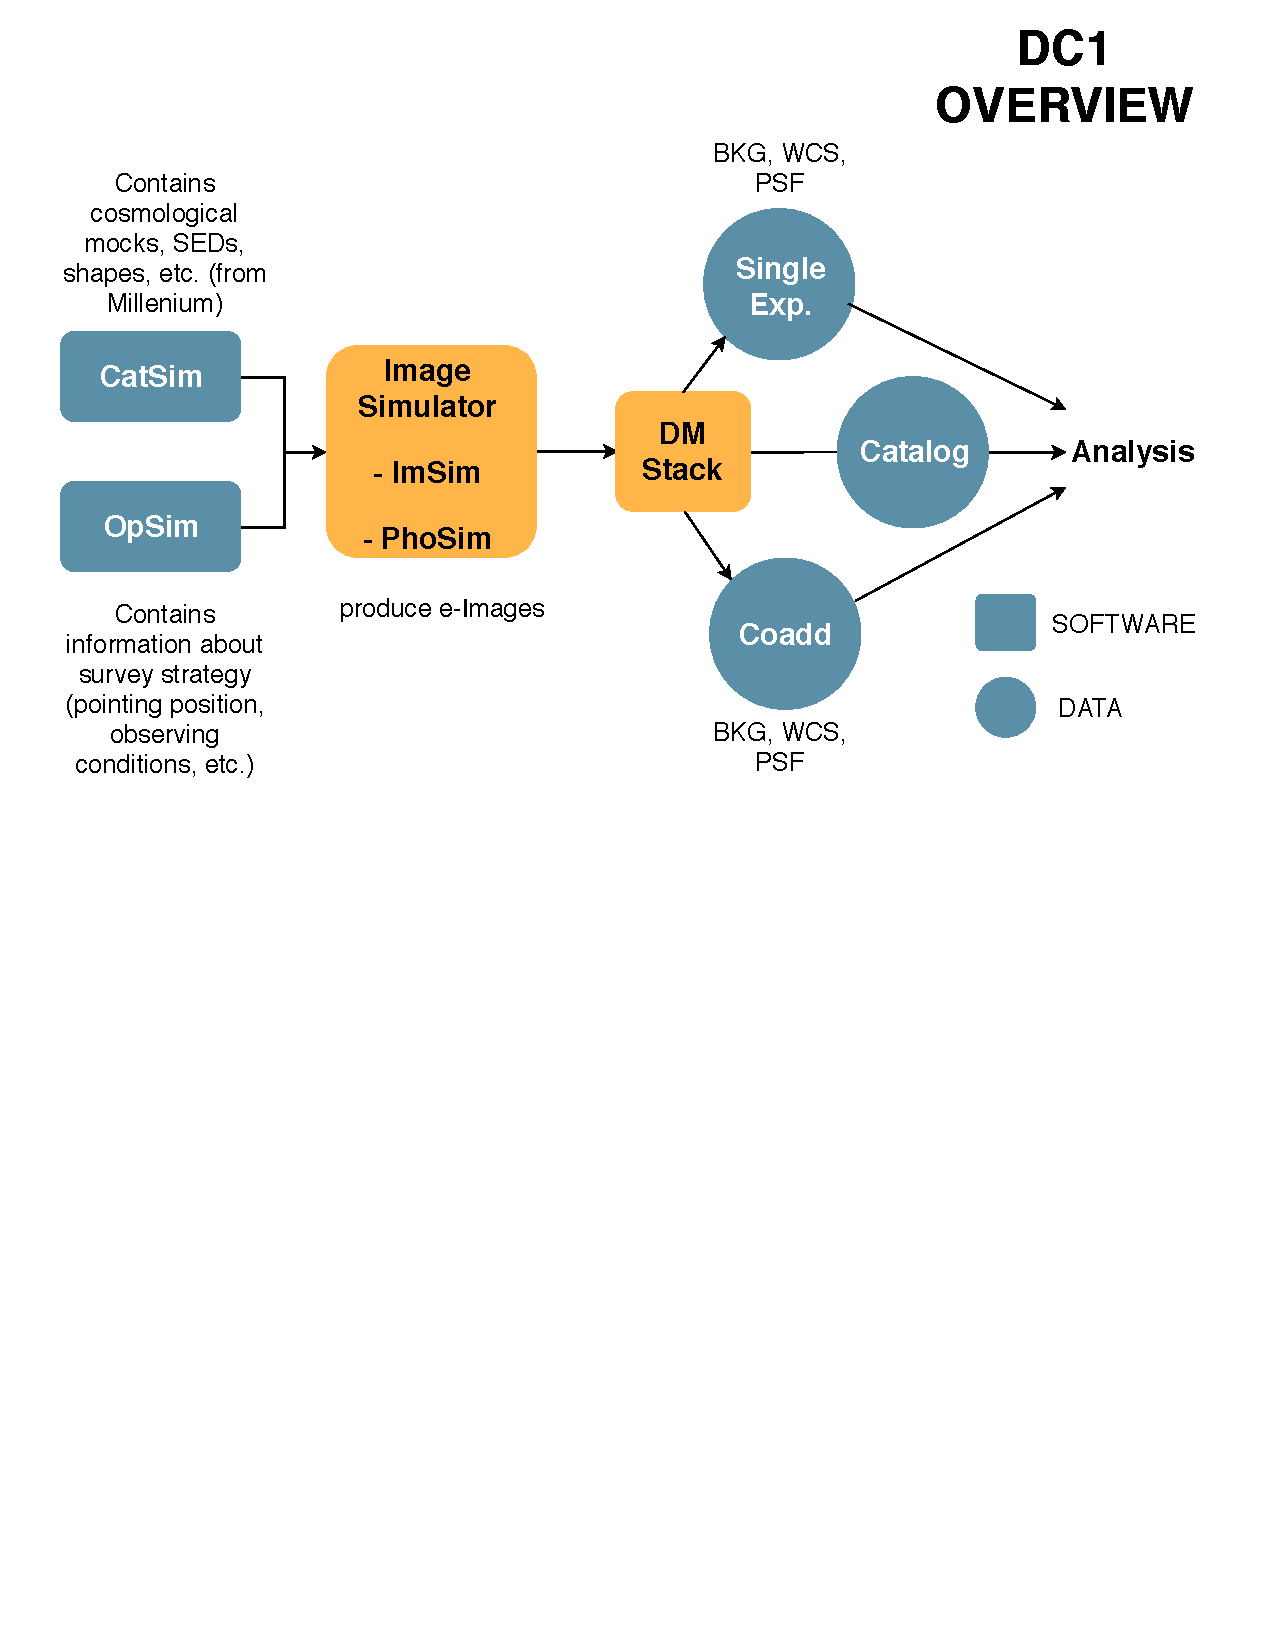
\includegraphics[trim={1cm 1cm 1.0cm 0.5cm}, 
clip, width=1.0\columnwidth]{dc1_workflow}}
\end{verbatim}
\as{file not in repo}
\caption{Workflow diagram for full data simulations. The image simulation step produces synthetic raw observations from a known truth catalog based on N-body simulations and simulated observing conditions. These data, in the same format as actual observations from the LSST telescope are processed by the data management to first generate calibrated single exposure images. These are calibrated both astrometrically and photometrically and are fed again into data management stacks that produces the image co-adds and a catalog of detected static sources.  \textcolor{red}{Get rid of phosim??}.
  \as{This file seems to be missing from the repo, but from the pdf version
    you send around, it needs work: The output of Image Simulator are raw exposure (eframes or whatever they are called). This is its own circle and it is is importnat. This then feeds into DM, which produces \emph{Calibrated single exposures}. These are then fed again into DM that produces a Co-add and catalog. I've also changed caption. You also need to have a side-arrow for transients for completion. }
}

\label{fig:dc1_workflow}
\end{figure}


\section{Image generation: input catalog}
\label{sec:inputs}
Image simulations allow us to study in detail the detection and deblending properties of a given image-processing pipeline. For example, if we produce images using an object catalog with random positions uniformly distributed across the sky, as well as uniformly random shapes and fluxes, we can get information about detection efficiencies as a function of flux.  However, the information about blending will not be realistic and we will not be able to capture some correlations present in real data. On the other hand, using N-body simulations as the input to generate artificial images allows us to study all the aforementioned effects. This is why we used the \texttt{CatSim}~\citep{2010SPIE.7738E..1OC,2014SPIE.9150E..14C} catalog as our input.  \texttt{CatSim} is a set of simulations provided by the LSST Simulations Team representing a realistic distribution of both Milky Way and extra-galactic sources. In particular, the extra-galactic catalog contains galaxies covering the redshift range $0 < z < 6$ in a 4.5$\times$4.5 degree footprint. The galaxies are generated by populating the dark matter haloes from the Millennium simulation~\citep{2005Nature.435.629S} using a semi-analytic baryon model described in \citet{2006MNRAS.366..499D} including magnitudes BVRIK and bulge-to-disk ratios. For all sources, a spectral energy distribution (SED), is fit to the galaxy colors using \citet{2003MNRAS.344.1000B} spectral synthesis models. Fits are undertaken independently for the bulge and disk and include inclination dependent reddening. Morphologies are modeled using two S\'{e}rsic profiles~\citep{1963BAAA....6...41S} and a single point source (for the AGN). Half-light radii for the bulge components are derived from the absolute-magnitude vs half-light radius relation given by \citet{2011A&A...534A...3G}. Stars are represented as point sources and are drawn from the Galfast model~\citep{2008ApJ...673..864J}. More information about these catalogs can be found at the LSST Simulations webpage\footnote{\url{https://www.lsst.org/scientists/simulations/catsim}}.

For the Data Challenge 1 (DC1), we chose a nominal field at \as{give ra dec coordinates}. This field has a galatic latitude of \as{fill} and a dust extinctions of \as{fill} an thus represent what a typical LSST dataset will be. The \texttt{CatSim} catalog was tiled to generate a $\sim 40$ deg$^{2}$ footprint covering 4 LSST full focal plane pointings. . This approach introduces a periodicity that induces extra correlations in our sample, however, this is not a major defect as we are unable to measure correlations on relevant scales with any useful precision.

After tiling, the input catalog contains approximately $63.1$ million sources, of which 97\% are galaxies whose redshift and magnitude distributions are depicted in \figref{catalog_plots} and remaining objects are stars. We simulate images in $r$-band to the LSST full depth ($10$ years). The final footprint can be seen in \figref{footprint}. We simulate observations within this footprint using the \texttt{minion\_1016}\footnote{\url{https://www.lsst.org/scientists/simulations/opsim/opsim-v335-benchmark-surveys}} simulated observing cadence generated with the LSST Operations Simulator (OpSim)~\citep{2014SPIE.9150E..15D}. This gives \as{fill} pointings of our field over 10 years.

\begin{figure}
\centering
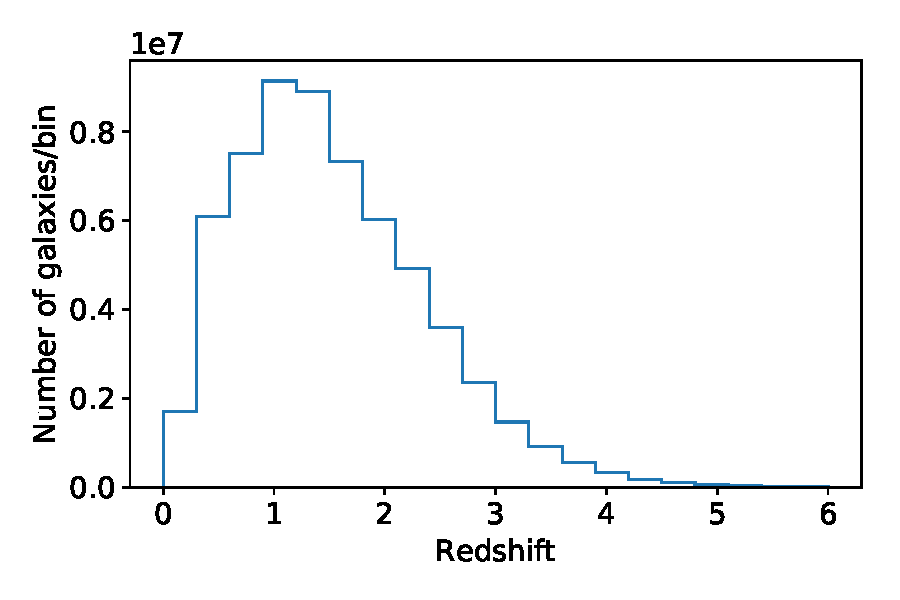
\includegraphics[width=0.9\columnwidth]{N_z_DC1.pdf}
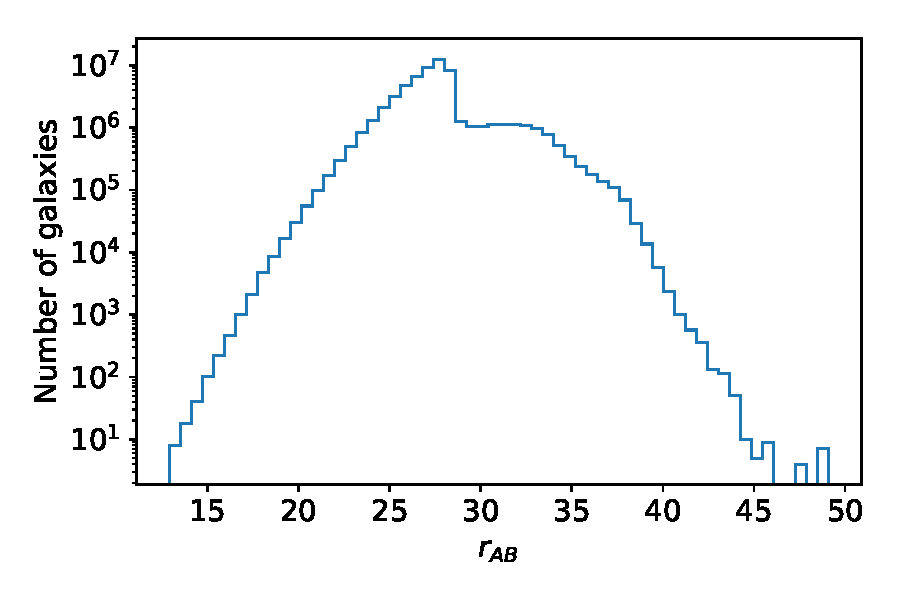
\includegraphics[width=0.9\columnwidth]{N_m_DC1.pdf}
\caption{Redshift (top) and magnitude (bottom) distribution for the galaxies used as inputs for the Data Challenge 1 simulations. In the magnitude distribution we include, as references, the typical depth for a single exposure (red dashed line) and the median depth in the DC1 dithered simulation (black dashed-dotted line).}
\label{fig:catalog_plots}
\end{figure}

\section{Dither strategy}
\label{sec:dithering}

As mentioned in \secref{design}, we use OpSim's output, which contains a realization of the LSST observing cadence and the survey footprint. Since OpSim divides the sky with hexagonal tiles, the nominal telescope pointings lead to overlapping regions across adjacent tiles that are observed more often than the non-overlapping part of the field-of-view (FOV), resulting in depth non-uniformity on the scale of $\sim$1 degree and consequent systematic uncertainties \citep{2016ApJ...829...50A}. In an effort to mitigate these effects, we implement \textit{dithers} -- offsets in the nominal telescope pointings. Specifically, here we use \textit{large}, i.e., as large as the FOV, random translational dithers, implemented after every visit, and random rotational dithers implemented after every filter change. The specific translational dither strategy is chosen based on a more extensive study of the various (translational) dither strategies in \citet{2016ApJ...829...50A}, where random dithers after every visit are found to be amongst the most effective.

For our purposes, we consider both the undithered and the dithered observing strategy. For the dithered strategy, some visits will contain sensors that fall out of the DC1 region; these sensors were not simulated in order to save computational resources.
\as{But for dithered option, presumably the right thing to do would be also considered pointings that are not nominally on our field, but happened to be partially dithered into it. Otherwise, the total depth of the undithered is higher as you never throw anything away? Explain.}



\section{Image generation and processing}
\label{sec:image_generation_pipeline}
% ---------------------------------------------------------------------

The artificial generation of astronomical images is a complex and computationally demanding process. In the recent
years, there have been major efforts in the community to create software that enables the generation of astronomical images, with various choices made in terms of level of complexity and fidelity, and computational efficiency, such as \texttt{UFIG}~\citep{2016ApJ...817...25B}, and \textsc{PhoSim}~\citep{2015ApJS..218...14P}. In our case, we model the input sources using imSim\footnote{\url{https://github.com/LSSTDESC/imSim}}\textcolor{red}{Add reference Walter et al., in prep??}, which internally uses \textsc{GalSim}~\citep{2015A&C....10..121R} as a library for image rendering, and uses LSST-specific information (e.g., about the geometry of the CCDs and the focal plane, the system throughputs in the different bands, etc.) to generate LSST-like images.
\as{Are we completely ignoring phosim runs here then? I think we should at least motivate imsim as a fast version of phosim. I'd say we did both, but say that in this first paper we are focusin on imsim results}


\subsection{imSim}
\label{sec:imsim_pipeline}

imSim is an open-source image simulation software package that uses GalSim with a modular approach. It allows the user to change the level of realism of the simulations by changing the complexity of PSF, background and source modeling. In particular, we used a pre-release version specifically meant to perform the DC1 simulations: \texttt{imSim v.0.1.0}\footnote{\url{https://github.com/LSSTDESC/imSim/releases/tag/0.1.0}}.


For DC1, we simulate each CCD of the focal plane individually, and instead of the planned two 15-seconds exposures~\citep{Overview}, we generate a single image with a 30-second exposure time to simplify the data handling. We omit instrumental effects and variability in the optical model across the focal plane. Since this is the first DESC data challenge, we want to ensure that we are able to generate and process the simplest cases, and then, build upon this base, increasing the complexity and level of realism for future data challenges. Our sky brightness model is based off the \citet{1991PASP..103.1033K} model provided by OpSim, refined by the detailed wavelength dependence of the phenomenological model from~\citet{2016SPIE.9910E..1AY}. The PSF model is a Gaussian for the system with a full-width half-maximum airmass dependence\footnote{From LSST-20160 eqn.~(4.1) \rachel{should link to this document / name it}}\textcolor{red}{LSST-20160 is not public...}, this is done to mimic the degradation in the image quality due to, e.g., gravity load\footnote{See LSE-30~\url{http://ls.st/lse-30} p.80}. A Kolmogorov profile is used to model the atmosphere which is also airmass dependent\footnote{From LSST-20160 eqn.~(4.2)}. The airmass, $X$, depends on the angular distance to the zenith, $Z$, as follows~\citep{1991PASP..103.1033K}:

\begin{equation}
X = (1 - 0.96\sin{Z})^{-0.5}.
\end{equation}
imSim can generate three different types of objects: stars, which are modeled as PSF-like objects; galaxies, which are modeled as composite (bulge plus disk) S\'{e}rsic profiles~\citep{1963BAAA....6...41S} using
the parameters given by CatSim; and AGNs which are also modeled as point sources and, for simplicity, without any variability. Future versions of imSim will have the ability to generate more complex galaxy morphologies. The brightness for these sources is computed using the magnitudes from CatSim, which are converted to counts using the latest version of the LSST throughputs\footnote{\url{https://github.com/lsst/throughputs}}. We clip the objects at magnitude 10 in order to improve the computational efficiency.

The final products of this pipeline are FITS images with information about the observing conditions. We generated more than 200,000 images in total (including both the \textit{dithered}, and \textit{undithered} fields). The average time to simulate each CCD is $\sim 4300$ seconds and the total production time is $\sim 270,000$ CPU-hours.

\subsection{Image processing}
\label{sec:image_processing_pipeline}

The outputs of these simulations are then processed using the LSST data management (DM) software stack~\citep{Overview,ScienceBook,WhitePaper,2018PASJ...70S...5B,2015arXiv151207914J} using version 13.0\footnote{\url{https://pipelines.lsst.io/releases/v13_0.html}}. The DM stack is an open-source, high-performance data processing and analysis system intended for use in optical and infrared survey data. The code can be found at \url{dm.lsst.org} and \url{pipelines.lsst.io}. The raw, uncalibrated single exposures are used as inputs. The software performs the reduction, detection, deblending and measurement on individual visits. It then combines the single-visit images to produce the so-called coadds. The DM stack provides calibrated images and source catalogs for the individual visits and coadds stored in \texttt{FITS} files. In total, we detect and measure $\sim 10.6$ (9.7 for the undithered simulation) million objects with position, flux and shape information. We activated optional extensions for the pipeline to include \texttt{CMODEL} fluxes (see \cite{2018PASJ...70S...5B} for more details) and \texttt{HSM} shapes~\citep{2003MNRAS.343..459H,2005MNRAS.361.1287M}.
\textcolor{red}{Ping Jim Chiang/Chris Walter/Tom G./Tony J.? to write something about the processing workflows for DC1.}
An example coadd cutout is shown in \figref{coadd_example}.

\rachel{Big picture comment: we don't talk at all about any of the software that drove these things - workflows for the DM processing etc.  Is that sufficiently trivial that it doesn't need to be mentioned?}

\begin{figure}
\centering
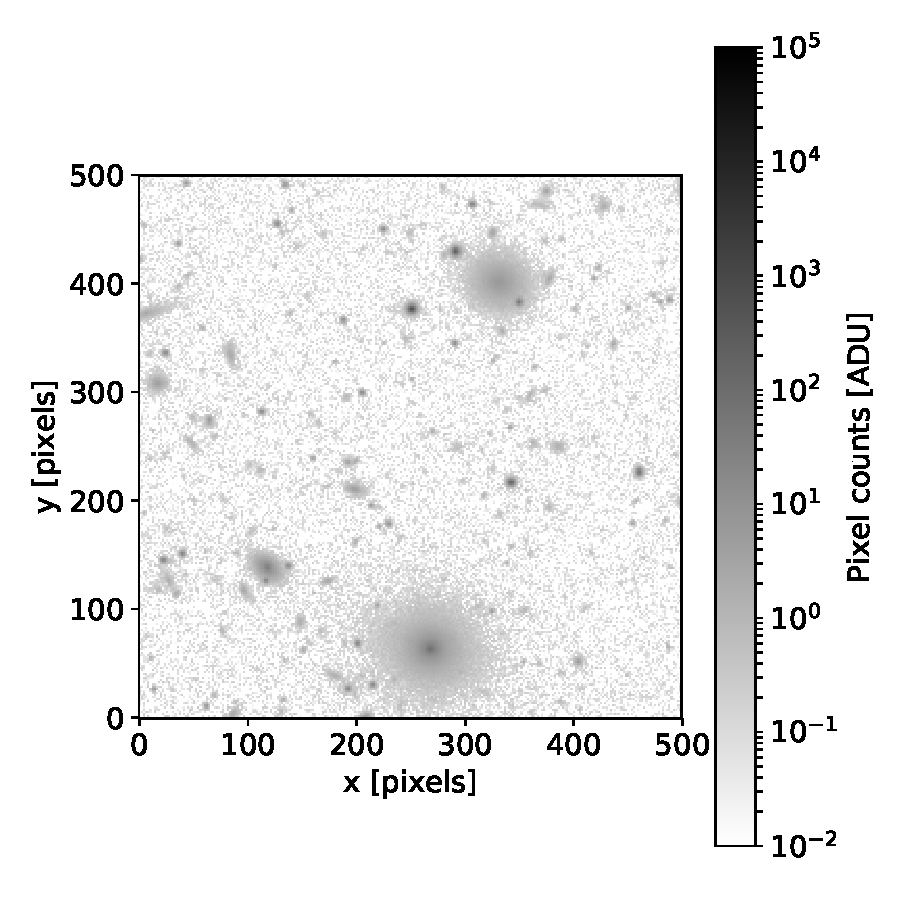
\includegraphics[width=0.9\columnwidth]{sample_coadd_DC1.pdf}
\caption{Example of a 500 $\times$ 500 pixel cutout from a full depth coadd showing the large density of objects in the LSST full-depth images.
\as{Change this figure as follows: make a three/four panel figure showing: i) the true sky (basically imsim run with noise and psf, etc switched off); ii) a raw uncalibrated image of the sky; iii) the single calibrated exposure if sufficiently different -- the scale should now how different units and you can draw line of const ra/dec to indicate astrometric calibration and iv) the 10yr coadd.}}
\label{fig:coadd_example}
\end{figure}

\section{Output catalogs and validation}
\label{sec:catalogs}
After being processed, the catalogs are stored at the National Energy Research Scientific Computing Center (NERSC)\footnote{\url{http://www.nersc.gov}} and accessible to DESC collaborators. We generate \texttt{pandas
dataframes}~\citep{mckinney-proc-scipy-2010} and databases for each one of the coadds and input catalogs, providing collaborators some flexibility in data access for their own analyses. As mentioned earlier, the output catalogs contain 10.6 (9.7) million objects covering an area
of $\sim$43 deg$^{2}$. The catalogs include information about position, size, shape and magnitude for every object. They include several flags that give information about the presence of interpolated/saturated pixels in the objects and whether or not these objects are close to the edge of a CCD.

In order to check the level of realism and the accuracy of the processed catalogs we perform several quality assurance tests. These tests will be performed in the dithered simulation, however, unless stated, the procedures and results are similar for the undithered simulation.

\subsection{LSST Science Requirements Document Key Performance Metrics}

After doing some basic sanity checks, we processed the output individual-visit catalogs through the LSST Project package \texttt{validate\_drp}\footnote{\url{dmtn-0008.lsst.io}, \url{https://github.com/lsst/validate_drp}}.
The \texttt{validate\_drp} package calculates the Key Performance Metrics (KPMs) from the LSST Science Requirements Document\footnote{\url{https://ls.st/LPM-17}}~\citep{LPM-17}, which we will refer to as LSST-SRD. This document contents science-driven requirements for LSST data products and we use it as a guide to check the status of our end-to-end pipeline. In addition, we will also validate our dataset using some of the requirements at the DESC Science Requirement Document~\citep[][DESC-SRD;]{2018arXiv180901669T}, which we will refer to as DESC-SRD.
 
By design, our simulations do not satisfy some of the requirements in the LSST-SRD, such as the number of filters in the surveyed fields (Filter complement in Table~\ref{tab:kpm_table}) or the number of filters (Nfilt) used in a given night because we only simulate images in $r$-band. On the other hand, our images automatically meet some criteria due to the design choices. For example, the maximum pixel size (pixSize) allowed in the LSST-SRD is 0.22 arcseconds and our simulations have a fixed pixel size of 0.2 arcseconds. Finally, some requirements in both the LSST-SRD and the DESC-SRD cannot be tested with these single-band images, we will ignore such tests in this work.

We start by checking the absolute astrometry by comparing the input and output catalogs. We find a mean (and median) deviation of 38 milliarcseconds between the input and measured positions. This is due to the fact that the corrections for proper motion were not present in the version \texttt{13.0} of the DM stack. However, this bias is still below the design specifications for the absolute astrometric performance of LSST as defined by the LSST-SRD, denoted by AA1, which is 100 milliarcseconds. This can be seen in~\figref{AA1}.

\textcolor{red}{Check with Chris and others: Why does the proper motion bias astrometry in one direction??}
\as{Probably because a few bright stars in this small field move in that one direction.}

\begin{figure}
\centering
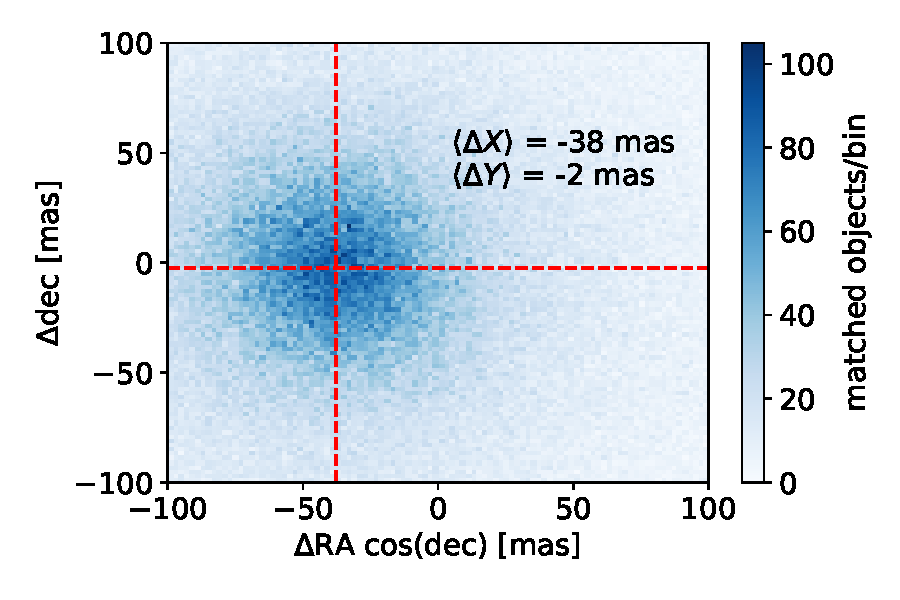
\includegraphics[width=0.9\columnwidth]{astrometric_residuals_single_visit_2d}
\caption{Astrometric residuals when comparing with the input catalogs for 500 randomly selected visits in the dithered simulation. We find a bias of 38 milliarcseconds in the measured right ascension due to uncorrected proper motion. We obtain similar results using the undithered simulation.}
\label{fig:AA1}
\end{figure}

We also validate the photometric repeatability by comparing the measured magnitude of bright unresolved objects across different visits, i.e., we select stars with signal-to-noise ratio (SNR) $> 100$. The photometric repeatability (PA1) is 6~mmag as measured by the interquartile range (IQR $\equiv$ 75th percentile minus 25th percentile) and is shown in \figref{validate_drp_PA1}. The minimum specification is 8~mmag so, our dataset and pipeline behave as required. The 6~mmag is dominated by a tail of scattered objects, see \figref{validate_drp_check_photometry}.

The photometric error model from \citet[][Eq. 4,5]{Overview} is \as{what units is this sigma in?}
\begin{eqnarray}
\sigma^2 = \sigma^2_{\rm sys} + \sigma^2_{\rm rand} \\
\sigma^2_{\rm rand} = (0.04 - \gamma) &10^{0.4(m-m_5)} + \gamma 10^{0.8(m-m_5)}
\label{eq:photometric_error}
\end{eqnarray}
where $\gamma$ describes noise from the sky and detector electronics, and the 5-$\sigma$ point-source depth is given by:
\begin{equation}
\begin{split}
m_5 = &C_m + 0.50 (m_{\rm sky} - 21~{\rm mag/{\rm arcsec}^2}) \\
&+ 2.5 \log_{10} (0.7{\arcsec}/\theta_{\rm eff}) \\
&+ 1.25 \log_{10} (t_{\rm vis} / 30~{\rm s}) - k_m (X-1)
\label{eq:photometric_m5}
\end{split}
\end{equation}
where $C_m$ summarizes the throughput of the telescope optics and camera, $m_{\rm sky}$ is the sky brightness, $\theta_{\rm eff}$ is the seeing, $t_{\rm vis}$ is the exposure time, $k_m$ is the airmass coefficient, and $X$ is the airmass.

Our fits find $m_5$ = 24.2~mag/arcsec$^2$ and $\gamma=0.038$ which are quite consistent with the \citet[][Table 2]{Overview} values of $m_5=24.35$~mag/arcsec$^2$, $\gamma=0.039$.  This demonstrates that we generate simulations of the telescope, detector, and sky in accordance with the \citet{Overview} estimates.\as{How is this possible? Wasn't the sky level completely off in the DC1 sims?}

Note that we find $\sigma_{\rm sys}=0$~mmag, which is consistent with the idealized simulations we run for DC1 with no additional systematic sources of errors. The LSST-SRD also includes criteria about the percentage of bright, unresolved sources (PF1$= 20\%$) with a photometric measurement deviation larger than a certain threshold (PA2 = 15 mmag). We check this by computing the fraction sources in~\figref{validate_drp_PA1} that deviate more than 15 mmag, obtaining PF1$=17\%$ in compliance with the requirements.

\begin{figure}
\centering
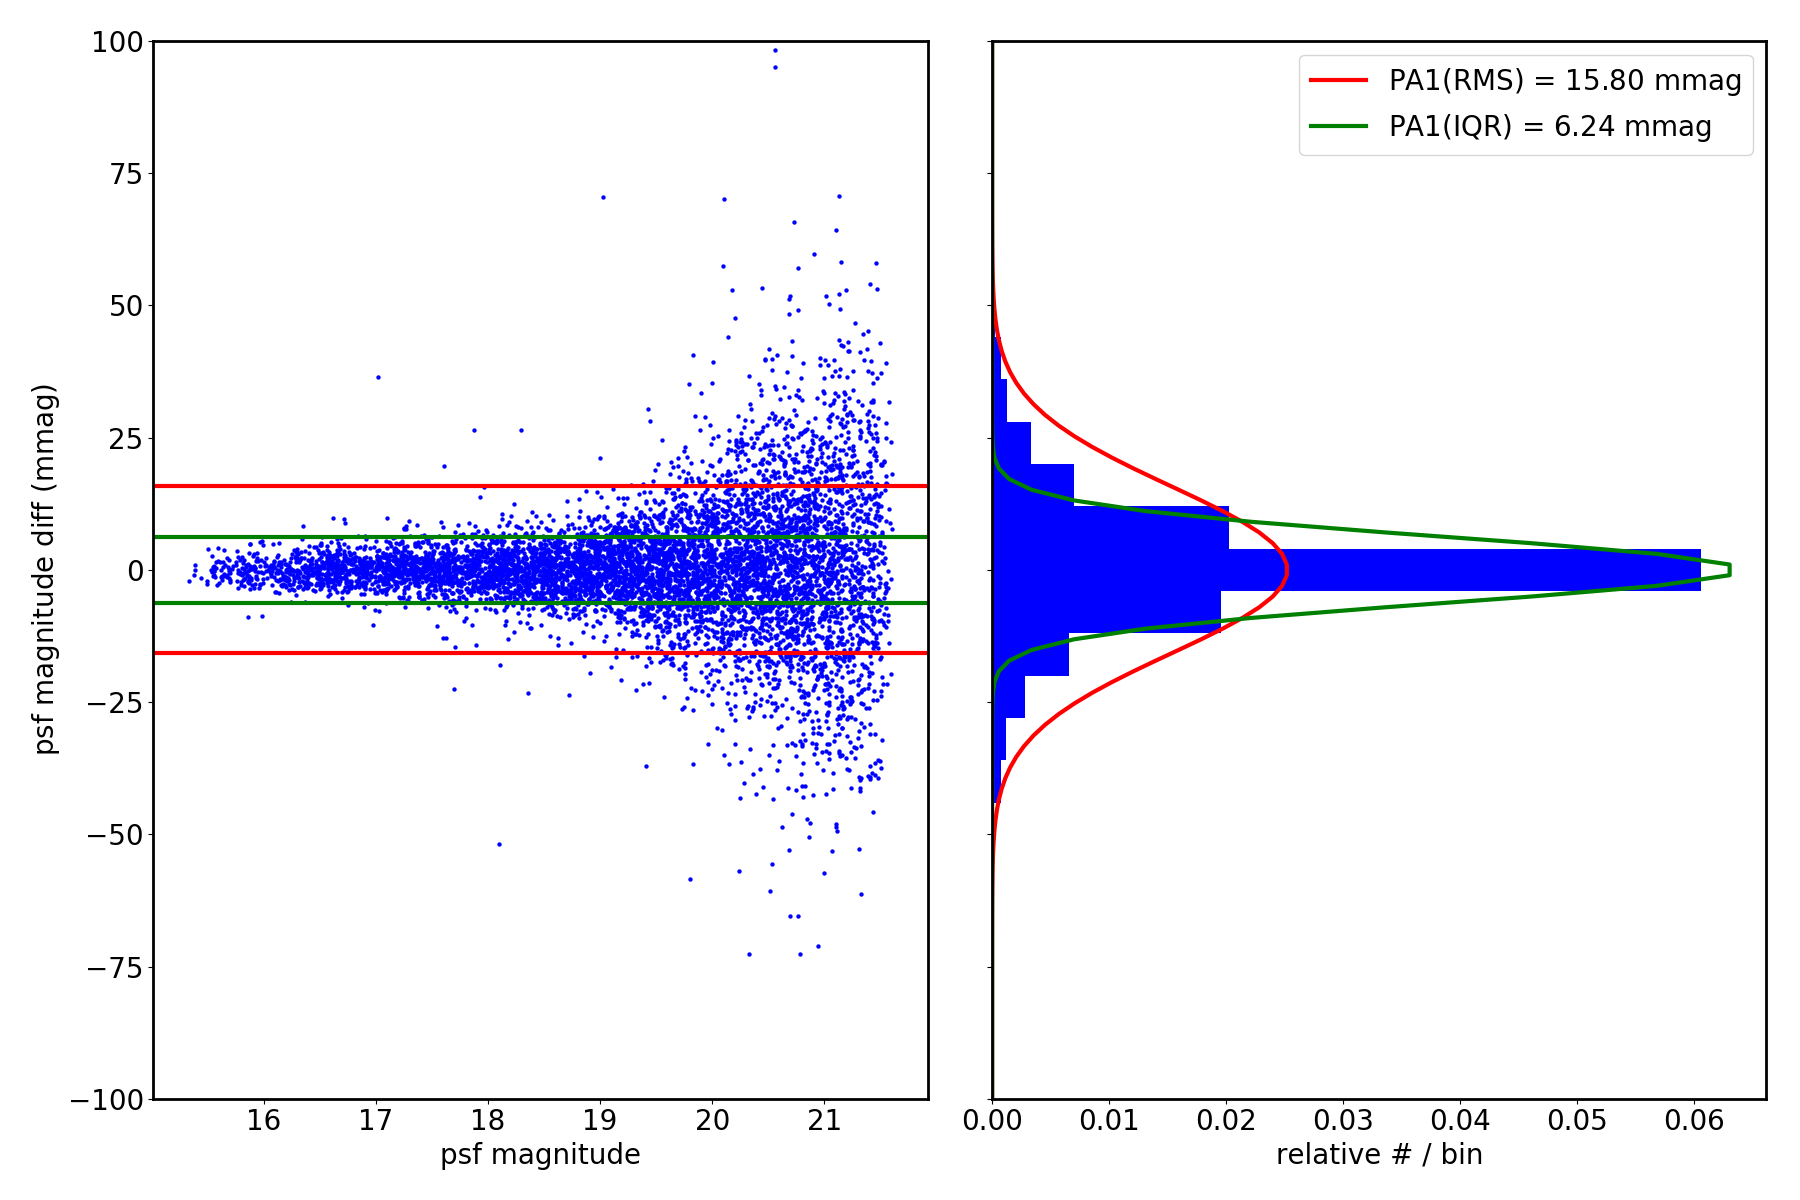
\includegraphics[width=0.9\columnwidth]{DC1-imsim-dithered_r_PA1.png}
\caption{(left) The magnitude difference of pairs of measurements of stars across visits for stars with a typical SNR $>100$.  (right) The histogram of these differences.  The Gaussian root mean square (RMS) is shown in red while the interquartile range is shown in green. Note that the distribution is more peaked than a Gaussian. The interquartile range (6.2~mmag) is {\em smaller} than the Gaussian RMS (15.8~mmag).}
\label{fig:validate_drp_PA1}
\end{figure}

\begin{figure*}
\centering
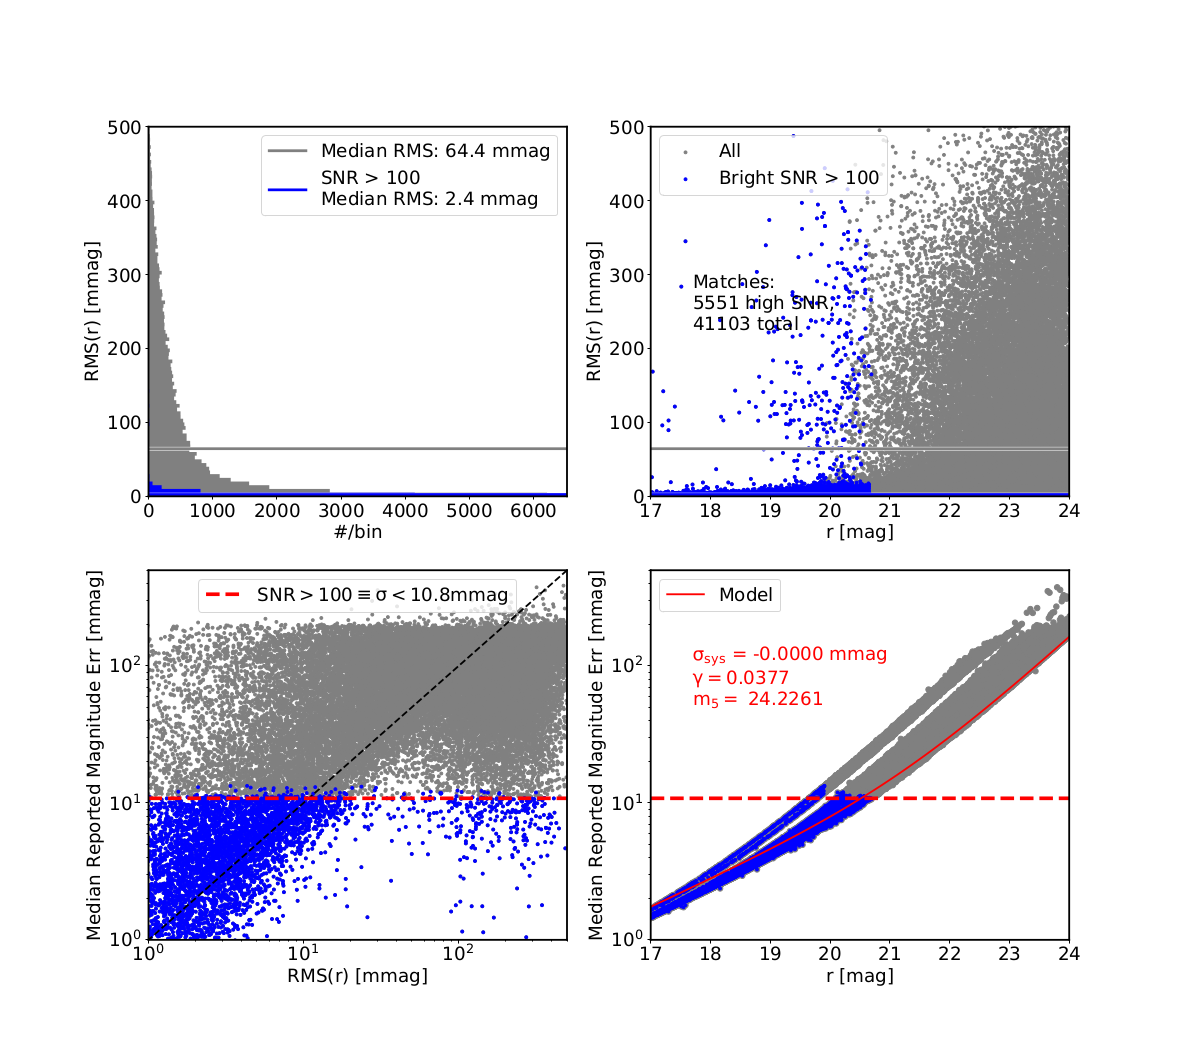
\includegraphics[width=1.8\columnwidth]{DC1-imsim-dithered_r_check_photometry.png}
\caption{Photometric performance in more detail.  (upper left) Horizontal histogram of the RMS distribution for each star for the full sample (grey) and ``bright'' sample (blue).  The blue sample is the same as that shown in Figure~\ref{fig:validate_drp_PA1}. (upper right).  Note that this RMS is the RMS of the measurements for a given star and so each entry in the histogram is one star. Thus, the median value here is 2.4~mmag, even thought the median of all RMS measurements in Figure~\ref{fig:validate_drp_PA1} was 15.8~mmag.  This difference is due to a population of objects that have a poor repeatability. (upper right) The RMS distribution as a function of magnitude of the star.  Here you can see the tight core of very repeatable measurements, along with a smaller population of objects with much higher scatter to their measurements. (lower left) Per-object median reported magnitude error by the pipeline versus the observed RMS over all of the measurements for an object.  Our $SNR>100$ cut is in the space of median reported error. (lower right) Per-object median pipeline-reported magnitude error versus object magnitude. 
{\bf TODO: MWV CLEANUP (1) title, (2) incorrect xlabel (should be \#/bin),  and "Filter name" extra text}
{\bf TODO: MWV  Are these higher scatter objects galaxies, stars in halos of bright stars, additionally added objects that were done inconsistently with the rest of the catalog?}
{\bf TODO: MWV  The lower-left plot has never actually made sense to me.  I should investigate this more.}
}
\label{fig:validate_drp_check_photometry}
\end{figure*}

We continue by checking that the zeropoints, $z_{p}$ fulfill the uniformity requirements specified in the LSST-SRD. More concretely, they should have show an RMS lower than 15 mmag (PA3) and no more than 20\% (PF2) of the images should have a deviation larger than 20 mmag (PA4). We randomly select 1000 sensor-visits and check the distribution of the zeropoints, depicted in~\figref{PA34}, finding that the RMS of the distribution is 37 mmag, not fulfilling the requirement. This is not worrisome since we are not interested in the colors of the sources given that we only have single band images. \as{You can't say things like this! This is not real data and we could have had other bands and then it would be worrisome!} We also find that 19\% of the sensors have a zeropoint that deviates from the median more than 20 mmag in compliance with the requirements. Finally, we compare input and output magnitudes and compute the median difference between both (PA6), finding it to be 17 mmag and smaller than the maximum allowed in the LSST-SRD (20 mmag). More details about how the matching between inputs and outputs was done in order to perform this test can be found in~\ref{ssec:matching}.

\begin{figure}
\centering
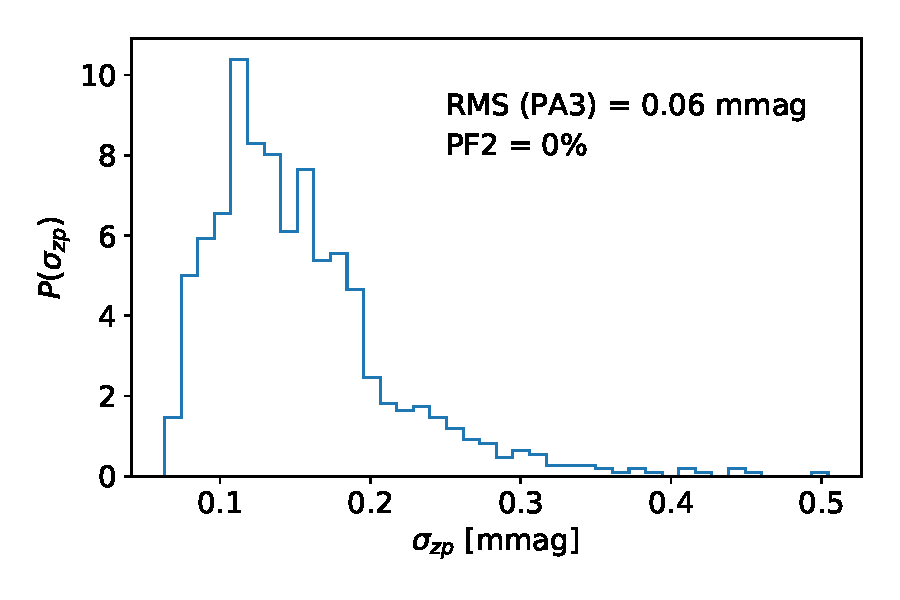
\includegraphics[width=0.9\columnwidth]{PA234.pdf}
\caption{Normalized distribution of the change in the zeropoint value, $\Delta z_{p}$ for 1000 randomly selected sensor-visits. We see that the distribution is quite asymmetrical and find that the RMS (PA3) is 37 mmag, larger than the requirements in the LSST-SRD (15 mmag). We also find that only 19\% (PF2) of the visits deviate from the median more than 20 mmag (PA4), in compliance with the LSST-SRD requirements.}
\label{fig:PA34}
\end{figure}

We now focus on checking the astrometric performance.  We show the detailed astrometric repeatability in \figref{validate_drp_check_astrometry}, where detected stars that are detected at different visits are matched and their astrometric residual is shown as a function of their SNR. The LSST-SRD sets astrometric requirements for stellar pairs at a separation $D$ in different exposures. The RMS of the separation between these pairs should not exceed AMx milliarcseconds and less than AFx \% of the sample should deviate more than ADx milliarcseconds from the median. AMx, AFx, and ADx are specified for pairs separated by D=5, 20 and 200 arcmin for x=1,2 and 3. The results of these checks can be found in~\figref{validate_drp_AMx}.

\begin{figure}
\centering
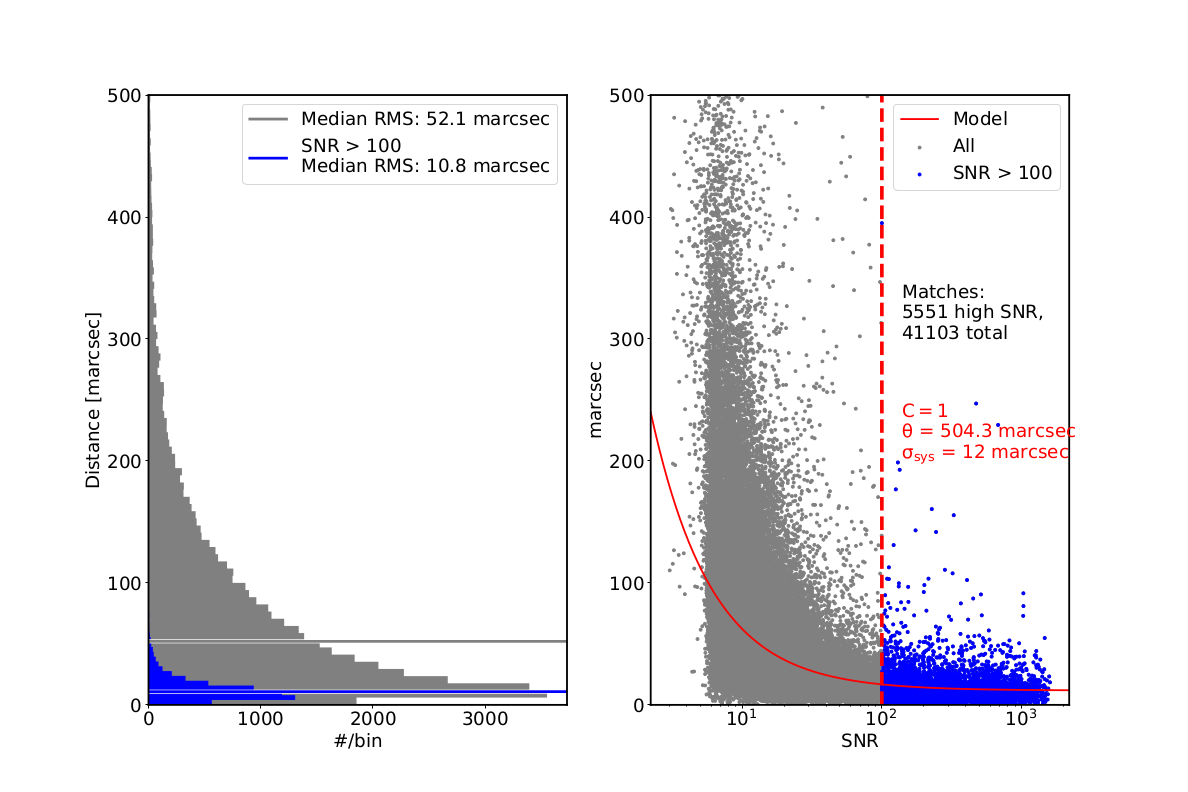
\includegraphics[width=0.9\columnwidth]{DC1-imsim-dithered_r_check_astrometry.png}
\caption{
Detailed astrometric performance.  (left) Histogram of the repeatability of distance between pairs of stars.  (right) Astrometric variation as a function of SNR.  We find a systematic floor of 12~milliarcsec.
{\bf TODO: MWV CLEANUP (1) title, (2) fix xlabel, which should be \#/bin}
{\bf TODO: MWV IS THIS HISTOGRAM DIFFERENT THAN THE check\_photometry histogram in terms of per-pair vs. per-object variation.}}
\label{fig:validate_drp_check_astrometry}
\end{figure}

\begin{figure}
\centering
\includegraphics[width=0.9\columnwidth]{{DC1-imsim-dithered_r_validate_drp.AM1_D_5_arcmin_17.0_21.5_mag}.png}
\includegraphics[width=0.9\columnwidth]{{DC1-imsim-dithered_r_validate_drp.AM2_D_20_arcmin_17.0_21.5_mag}.png}
\includegraphics[width=0.9\columnwidth]{{DC1-imsim-dithered_r_validate_drp.AM3_D_200_arcmin_17.0_21.5_mag}.png}
\caption{
Astrometric repeatibility: variation in distances measurement between pairs of stars at (top) 4-6$\arcmin$, (middle) 19-21$\arcmin$, (bottom) 199-201$\arcmin$.  AM(1,2,3) are the distance measurements, while AF(1,2,3) are the fraction of pairs lying outside the a specified limit AD(1,2,3).
The performance is excellent, with characteristic values all below the LSST-SRD levels.
{\bf TODO: MWV CLEANUP}}
\label{fig:validate_drp_AMx}
\end{figure}

In addition, the LSST-SRD sets some requirements in the minimum per-visit image depth for images with fiducial sky brightness of 21 mag/arcsec$^2$, exposure time of 30 s, airmass=1 and fiducial seeing (FWHM) of 0.7 arcseconds. In order to mimic this we select the visits that fulfill the following criteria:
\begin{itemize}
\item Altitude $> 80$ degrees.
\item $0.68\arcsec <$ seeing (FWHM) $ < 0.71\arcsec$
\item Sky-brightness (in $r$-band) $ \geq 21$ 
\end{itemize}LSST-SRD
We obtain a total of 520 sensor-visits fulfilling these criteria. We then compute the median 5-$\sigma$ depth following the methodology described later in this work and compare with the predicted depth by \texttt{OpSim}. After this, we check that the median of the depth distribution is larger the minimum depth (D1=DB1=24.3 mag) as defined in the LSST-SRD. We also check that no more than 20\% of the visits (DF1) have a depth lower than 24.0 (Z1) by computing the 20th percentile. The results of these checks are depicted in \figref{DF1_checks}. We find that the median of the depth distribution in the selected visits, $24.297 \pm 0.009$ mag, is compatible (within a standard deviation of the mean) with the minimum depth set in the LSST-SRD. We find as well that the 20th percentile 24.1 is larger than the minimum value (Z1) set in the LSST-SRD. We also check that in a given visit, the variation in the field-of-view is within the requirements. The LSST-SRD establishes that, in a representative visit with depth D1 no more than (DF2) 20\% of the field-of-view will be (Z2) 0.4 magnitudes brighter than the nominal (24.3). We select visit 2218486 since its median depth is 24.3. We find that the 20-th percentile is 24.29 fulfilling the criteria.

\begin{figure}
\centering
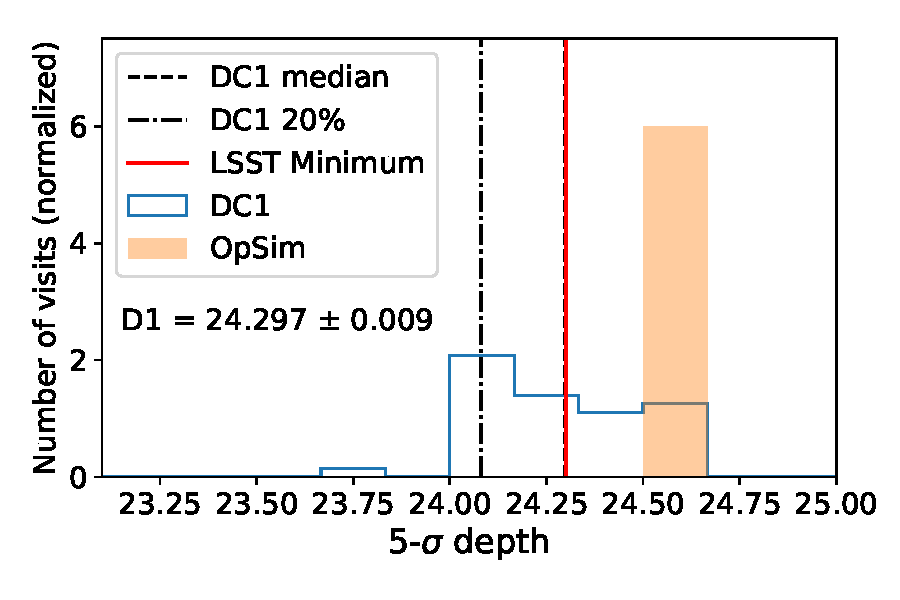
\includegraphics[width=0.9\columnwidth]{m5_goals}
\caption{Measured depth in visits with Altitude $>80$ deg., $0.68 \arcsec <$ seeing $ < 0.71 \arcsec$ and Sky-brightness (in $r$-band) $\geq 21$ (blue histogram) compared to the predicted depth by \texttt{OpSim} (solid orange histogram). The median of this distribution (dashed line) is very close to the LSST-SRD minimum depth D1=24.3 (red vertical line), the 20th percentile is also shown and we can appreciate that is larger than Z1=24.0 as established by the LSST-SRD.}
\label{fig:DF1_checks}
\end{figure}

The LSST-SRD also sets criteria regarding the maximum modulus of the PSF ellipticity, $|e|$,
for exposures with PSF-FWHM $\approx 0.69\arcsec$ and no more than 10 degrees apart from zenith, where $|e|$ follows the distortion definition~\citep{1991ApJ...380....1M}:
\begin{equation}
|e| = \frac{a^{2} - b^{2}}{a^{2}+b^{2}}
\end{equation}
were $a, b$ are the semi-major and semi-minor axes of the 
in particular, it requires that the median is no larger than 0.05 (SE1) and that no more than 10\% (EF1) of the images exceed 0.1 (SE2). Our analytic (and circularly-symmetric) PSF models should, by design, fulfill these criteria. However, we have to test if the reconstructed PSF also fulfills them. The PSF was reconstructed using the PSFEx~\citep{2011ASPC..442..435B} implementation in the LSST software stack. We tested this in the processed data by using the same 520 sensor-visits used to check the DB1 and DF1 criteria. We checked the modulus of the PSF ellipticity in the position of the detected objects in these visits accumulating them in the histogram shown in \figref{SE1_DC1}. We obtained that SE1=0.001 and SE2=0.002, way below the maximum values allowed by the LSST-SRD. In future data challenges, we plan to increase the complexity and realism of the PSF to be closer to the maximum values set by these requirements.

\begin{figure}
\centering
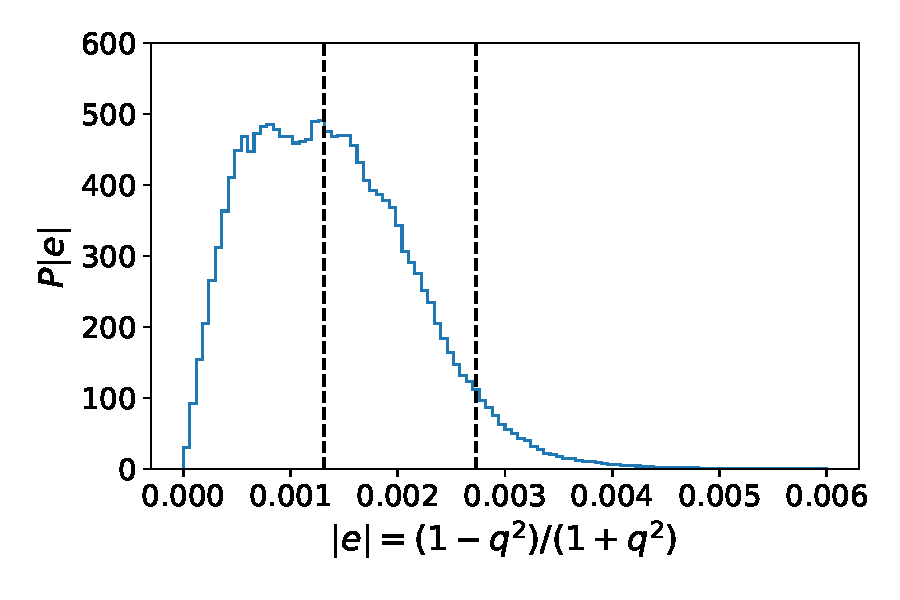
\includegraphics[width=0.9\columnwidth]{PSF_ellipticity_DC1}
\caption{PSF ellipticity distribution accumulated for 520 sensor-visits measured at the position of detected objects. The median (0.001) and 90th (0.002) percentiles are shown as the dashed lines. Note that these values are an order of magnitude lower than the specifications by the LSST-SRD (0.05 and 0.1, respectively).}
\label{fig:SE1_DC1}
\end{figure}

We also checked that, in these images, 85\% of the point-like sources flux is contained within $0.80\arcsec$ or less (SR1), 95\% within or less $1.31\arcsec$ (SR2) and 99\% within $1.81\arcsec$ (SR3) or less. In our case we obtain SR1$=0.64\arcsec$, SR2$=1.01\arcsec$ and SR3$=1.79\arcsec$. This was done by calculating the radius at which the PSF was at its 85th, 95th and 99th percentiles.

For weak lensing analyses, the correct modeling of the PSF is crucial~\citep{2004MNRAS.353..529H} and both the LSST-SRD and the DESC-SRD contain explicit requirements about the PSF residuals. In particular, the LSST-SRD states that using the full survey data the auto- and cross-correlations ($E_{1}, E_{2}, E_{X}$) of the PSF residuals over an arbitrary field-of-view should be below TE1 (3 $\times 10^{-5}$) for $\theta \leq 1$ arcmin, below TE2 ($3 \times 10^{-7}$) for $\theta \geq 5$ arcmin and no more than TEF (15) \% of the images will have median larger than TE3 ($6 \times 10^{-5}$) for $\theta \leq 1$ arcmin and, TE4 ($5 \times 10^{-7}$) for $\theta \geq 5$ arcmin. 

To check these criteria we calculate $E_{1}, E_{2}, E_{X}$ in using the definitions of the LSST-SRD:
\begin{eqnarray}
e_{1} = \frac{\sigma^{2}_{1} - \sigma^{2}_{2}}{\sigma_{1}^{2}+\sigma_{2}^{2}},\\
e_{2} = \frac{2\sigma^{2}_{12}}{\sigma_{1}^{2}+\sigma_{2}^{2}},\\
E_{1} (\theta) = \langle \delta e^{(i)}_{1}\delta e^{(j)}_{1} \rangle,\\
E_{2} (\theta) = \langle \delta e^{(i)}_{2}\delta e^{(j)}_{2} \rangle,\\
E_{X} (\theta) = \langle \delta e^{(i)}_{1}\delta e^{(j)}_{2} \rangle,
\end{eqnarray}
With $\sigma_{1}^{2}, \sigma_{2}^{2}$ are the second order moments of a source along some set of perpendicular axes and $\sigma^{2}_{12}$ is the covariance, $\delta e_{1}, \delta e_{2}$ are the residuals, and the angle brackets indicate averaging over all pairs of stars $i$, $j$ at a given angular separation $\theta$.

In practice, we compute the PSF-corrected moments of stars across the field of view using \texttt{TreeCorr}~\citep{2004MNRAS.352..338J}. Our findings are shown in \figref{TEx}. We can see that for $E_{1}$ and $E_{X}$ the TE1 criteria is fulfilled but the TE2 and others are not. For $E_{2}$ there is a residual flat correlation. \textcolor{red}{Check with Robert/Rachel: This is likely a result of the our analytic PSF input model having some residual shape that cannot be described by the Gaussian profiles that the DM stack used, more suitable for real data?} \as{Ok, we should think more carefully if this is the right test to perform, but it is possible that this failure is real in the sense that PSF modelling in DM is currently not sophisticated enough, so this is a real failure of the SRD}
\begin{figure}
\centering
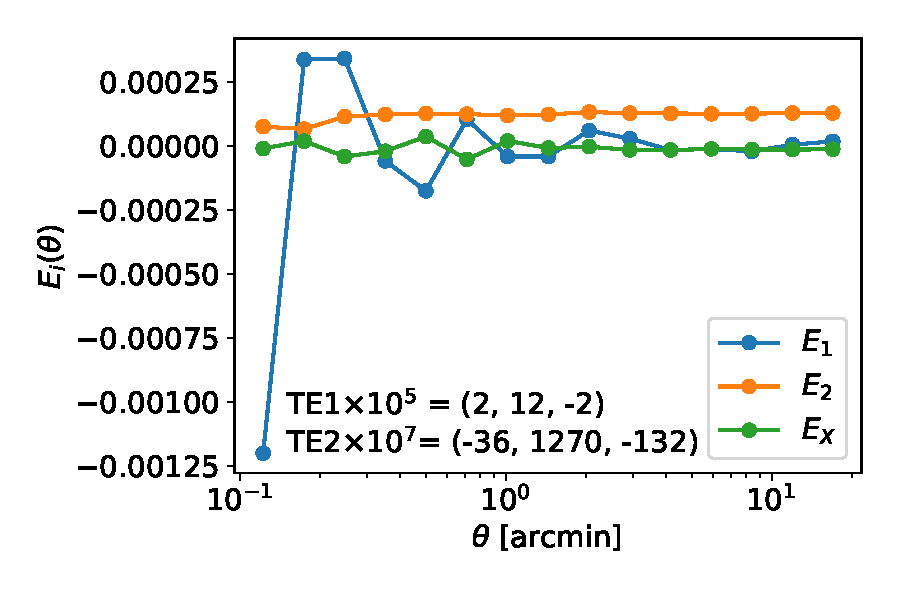
\includegraphics[width=0.9\columnwidth]{TEx}
\caption{Auto and cross-correlation functions, $E_{1}$ (blue), $E_{2}$ (orange), $E_{X}$ (green) of the PSF residuals as a function of the aperture angle $\theta$. We see that our data does not fulfill the LSST-SRD requirements.}
\label{fig:TEx}
\end{figure}

Finally, the DESC-SRD requires (WL4-Y10) that the systematic uncertainty in the PSF model defined using the trace of the second moment matrix should not exceed 0.1\% for full-depth (Y10) DESC weak lensing analysis. We randomly select 3000 visits, obtain the input and measured PSF, and measure the trace of the second order moments, $T$ with \texttt{GalSim}. We then compute the relative difference, $\Delta T/T$, obtaining the results depicted in \figref{WL4-Y10}. We find that our dataset shows that the standard deviation of the distribution is 0.05\% lower than the requirement.
\begin{figure}
\centering
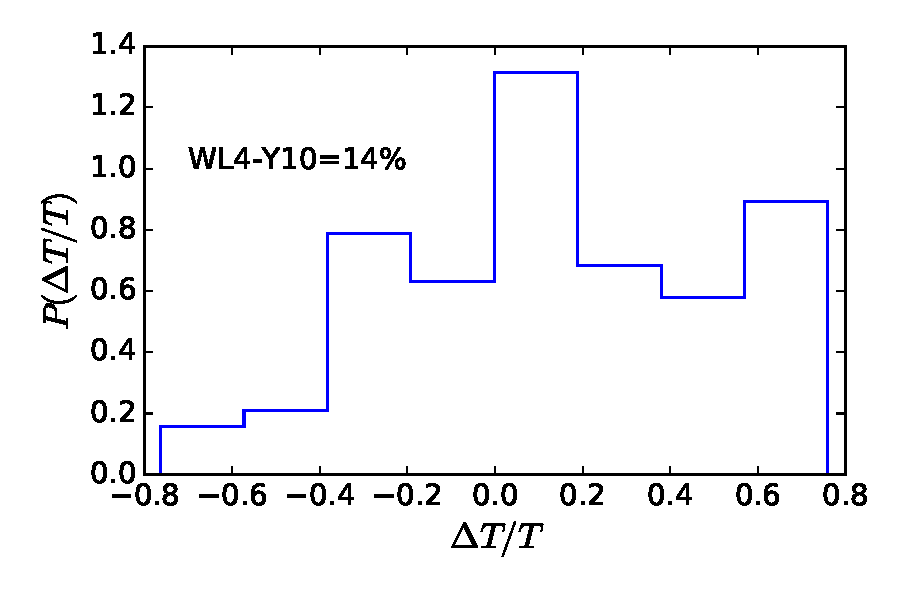
\includegraphics[width=0.9\columnwidth]{WL4-Y10}
\caption{Normalized distribution of the relative difference in the trace of the second order moments, $\Delta T/T$ between input and output PSF. We see that the standard deviation of the distribution (WL4-Y10) is 0.05\%, much complying with the requirement (0.1\%).}
\label{fig:WL4-Y10}
\end{figure}

We summarize our findings in Table~\ref{tab:kpm_table} and Table~\ref{tab:desc_srd_table}. We see that our images and catalogs pass most of the requirements by a good margin. We can also see that some of the criteria are not passing the requirements due to design choices and do not affect the science analyses that can be performed with this dataset. However, there is a big exception: the TEx requirements (correlations of the residual PSF ellipticity) which can prevent possible weak lensing analyses. \as{well, nobody wanted to do WL analysis using DM code anyway! } In any case, given that no cosmic shear signal was included in these simulations, the simplicity of the potential sources of systematic uncertainty for cosmic shear analyses, and the lack of photometric redshifts for the sources, this dataset does not offer any new science from the WL point-of-view and no WL analyses are performed on this work. 

\begin{table}[h!]
\centering
\begin{tabular}{|c|c|c|c|}
\hline
Quantity (LSST-SRD) & Minimum & DC1 & Passed\\
\hline
Filter complement & ugrizy & r & \textcolor{blue}{N}\\
Nfilters & 3 & 1 & \textcolor{blue}{N}\\
Nv1 & 184 & 184 & \textcolor{blue}{Y}\\
pixSize (arcsec) & 0.22 & 0.2 & \textcolor{blue}{Y}\\
AA1 (milliarcsec) & 100 & 20 & Y\\
PA1 (millimag) & 8 & 6 & Y\\
PF1 (\%) & 20 & 17 & Y\\
PA2 (millimag) & 15 & - & -\\
PA3 (millimag) & 15 & 37  & N\\
PF2 (\%) & 20 & 19 & Y\\
PA4 (millimag) & 20 & - & -\\
%PA5 (millimag) & 10 & 1.4 & check\\
PA6 (millimag) & 20 & 17 & Y\\
AM1 (milliarcsec) & 20 & 8 & Y\\
AF1 (\%) & 20 & 13 & Y\\
AD1 (milliarcsec) & 40 & - & -\\
AM2 (milliarcsec) & 20 & 4 & Y\\
AF2 (\%) & 20 & 9 & Y\\
AD2 (milliarcsec) & 40 & - & -\\
AM3 (milliarcsec) & 30 & 7 & Y\\
AF3 (\%) & 20 & 2 & Y\\
AD3 (milliarcsec) & 50 & - & -\\
%Fleak (\%) & 0.02 & 0 & \textcolor{blue}{Y}\\
%FleakTot (\%) & 0.1 & 0 & \textcolor{blue}{Y}\\
D1 (mag) & 24.3 & 24.3 & Y\\
DF1 (\%) & 20 & - & -\\
Z1 (mag) & 24.0 & 24.1 & Y\\
DB1 (mag/r-band) & 24.3 & 24.3 & Y\\
DF2 (\%) & 20 & - & -\\
Z2 (mag) & 0.4 & 0.1 & Y\\
%S1 (0.44) & 0.59 & check & check\\
%S1 (0.60) & 0.72 & check & check\\
%S1 (0.80) & 0.89 & check & check\\
%SF1 (\%) & 10 & check & check\\
%SX & 1.2 & check & check\\
%SXE & 0.59 & check & check\\
SE1 & 0.04 & 0.001 & Y\\
EF1 & 10 & - & -\\
SE2 & 0.1 & 0.002 & Y\\
SR1 (arcsec) & 0.80 & 0.64 & Y\\
SR2 (arcsec) & 1.31 & 1.01 & Y\\
SR3 (arcsec) & 1.81 & 1.79 & Y\\
TE1 & $3 \times 10^{-5}$ & $1.2\times 10^{-4}$ & N\\
TE2 & $3 \times 10^{-7}$ & $1.3\times 10^{-4}$ & N\\
TEF & 15\% & - & -\\
TE3 & $6 \times 10^{-5}$ & - & N\\
TE4 & $5 \times 10^{-7}$ & - & N\\
\hline
\end{tabular}
\caption{Table with the Key Performance Metrics (KPMs) that we used to check the quality of our end-to-end pipeline. The criteria that are passed or not due to design choices are shown in blue. We mark with dashes the quantities that we use as auxiliary to compute some of the criteria, e.g., we use EF1 to compute SE2.}
\label{tab:kpm_table}
\end{table}

\begin{table}[h!]
\centering
\begin{tabular}{|c|c|c|c|}
\hline
Quantity (DESC-SRD) & Maximum & DC1 & Passed \\
\hline
WL4-Y10 (\%) & 0.1 & 0.05 & Y\\
%WL5-Y10 (\%) & 0.1 & N/A & N/A\\
\hline
\end{tabular}
\caption{Criteria from the DESC-SRD tested in the DC1 simulation. This document also includes other criteria that cannot be tested with our data but will be relevant for future data challenges.}
\label{tab:desc_srd_table}
\end{table}

%\rachel{Is this all the KPMs?  I thought some have to do with PSF model quality, etc.}
%\rachel{Note that there are many figures associated with this subsection, but the text doesn't actually refer to or discuss any of them.}

\section{Data selection and masking}
\label{sec:data_selection}
In this section, we describe how we take advantage of the fact that we have full knowledge about the simulated sources in order to get a ``clean" data sample, we also describe the catalog mask and the maps generated for the different observational effects present in the simulation. Unless explicitly stated, the procedures and selections made in this section will be performed in both the dithered and undithered simulations.

\subsection{Matching inputs and outputs}
\label{ssec:matching}

Using end-to-end simulations, one can potentially trace each measured photon to its corresponding source and fully characterize the image generation and measurement processes. In practice, this is very difficult to do because, not just because  of the large data overhead, but because the entire data reduction pipeline is built around pixelated images rather than tagged photon counts.

Nevertheless, the output catalog is a noisy representation of the underlying true catalog and we need to find a way to connect the two. 
The simplest way to connect two catalogs is by using the positions of the objects in the sky. This approach has been extensively used in the literature~\citep{1977A&AS...28..211D,1983Obs...103..150B,1986MNRAS.223..279W} and performs reasonably well when blending is low (i.e, when the amount of overlapping sources in the image is low). However, when blending is high, this approach might be not be sufficient. Then, matching other quantities like flux or shape can become useful~\citep{2008ApJ...679..301B}.

We compare two different matching strategies: positional matching, where we find the objects in the truth catalog closest to the detected objects, which we will refer to as \textit{pure spatial matching} and will denote as \textsf{S}; and positional matching with magnitude matching, which we will refer to as \textit{spatial+magnitude matching} and denote as \textsf{S+M}, where for each detected object we find objects from the input catalog that lie within a three pixel radius ($0.6 \arcsec$). After this, we select the object that is closest in magnitude as long as the difference in magnitude is less than a certain threshold. In our case, we conservatively choose $1.0$. Using this approach, if none of the neighbors fulfill these conditions, the detected source is considered unmatched. Note that in the case of pure spatial matching all sources are matched to an object in the true catalog.

In both cases, we build a \texttt{KDTree}~\citep{scikit-learn} using the positions of detected objects with \texttt{detect\_isPrimary=True} which ensures that the source has been fully deblended and was detected in the inner part of the coadd regions (see~\citet{2018PASJ...70S...5B} and ~\citet{2018PASJ...70S..25M} for more details). In order to speed up the processing and to reduce the usage of computational resources we build the \texttt{KDTree} using output sources from 30 randomly selected coadd regions (patches) in the dithered simulation (the undithered simulation yields the same results and conclusions) containing 975,605 detected sources fulfilling the aforementioned condition (we will refer to these as primary outputs or primary detected sources). Using this sample, we find that 95\% of these sources are matched using the spatial+magnitude matching (by construction all of them are matched using the pure spatial matching approach). An interesting metric to check is the fraction of primary detected sources that have been matched to the same exact object in the input catalog, which we will denote as $f_{\mathrm{multi}}$. This is an unusual occurrence, however, imagine the case where an spurious fluctuation has been marked as a source, this fluctuation is a primary detected source but has no counterpart in the input catalog. Another example are bright objects that have been shredded and are detected as several fainter sources. We find that these kind of matches is $\sim 100$ times more likely to happen using the pure spatial matching ($f_{\mathrm{multi}} = 3 \times 10^{-3}$) than in the spatial+magnitude matching ($ f_{\mathrm{multi}} = 2 \times 10^{-5}$). This is expected because, in the cases where the primary detected source is a random fluctuation or a shredded source, it is unlikely that the measured flux is close to the flux of a neighboring source thus producing an unmatched source in the case of using spatial+magnitude matching. We also find that both approaches select the same best matching source in the input catalog for only 68\% of the primary detected sources for which we found a suitable match. These differences can be due to several reasons, e.g. objects with a poorly determined centroid positions that are close to other objects in the input catalog (remember that the input catalog contains objects up to $r=28$), objects with poorly determined fluxes (low SNR), etc.




We compare as well the astrometric and photometric residuals using both approaches in~\figref{matching_comparison}. We can see that the median astrometric residuals are similar in both cases and that the search radius (3 pixels=600 mas) for the spatial+magnitude matching is large enough to map the overall distribution. On the other hand, the resulting median photometric residual seems strongly biased in the case of using just pure spatial matching, and the scatter is very large as shown by the error-bars. However, in the case of spatial+magnitude matching, the median residuals and their error-bars are smaller, as expected given the maximum magnitude threshold. We can see that in this case the biases are still significant. This can be mitigated using a smaller tolerance in magnitude (for example using 0.5 mag instead of 1 mag) but that implies an overall reduction of the number of matched primary detected sources. Finally, taking a look at the magnitude difference between inputs and outputs of individual matched sources using the spatial+magnitude technique, we can see that this distribution is centered around zero, except for very bright sources ($r < 17$), where saturation prevents us from having an accurate determination of the fluxes. 

\begin{figure}
\centering
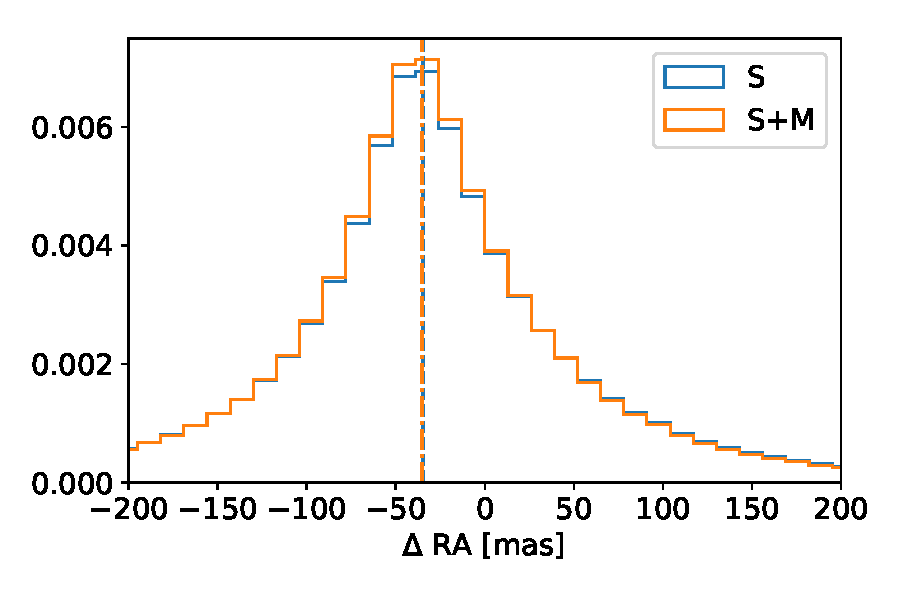
\includegraphics[width=0.9\columnwidth]{astrometry_residual_comparison}
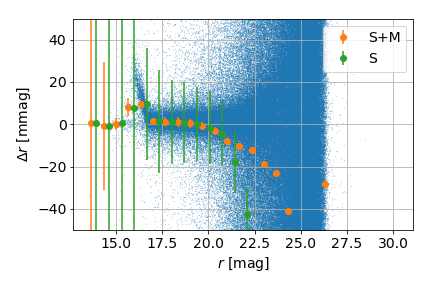
\includegraphics[width=0.9\columnwidth]{photometry_residual_comparison}
\caption{Top: Normalized distribution of measured astrometric residuals (in the RA axis but similar results are found for the Dec. axis) for pure spatial matching (blue) and spatial+magnitude matching (orange), the median values of each distribution are marked by dashed lines and dashed-dotted lines respectively. Bottom: Median per-bin photometric residual as a function of measured magnitude for pure spatial matching (green), and spatial+magnitude matching (orange) using 30 magnitude bins between $r$-band magnitude 10 and 30. We also show the individual residuals for the matched objects using spatial+magnitude matching (blue dots).}
\label{fig:matching_comparison}
\end{figure}

At the end of the day, different matching techniques have different potential applications and strengths. In our case, we are going to use these matching techniques to provide a clean (flux-limited) sample to perform two-point clustering analyses. Given that magnitude precision and accuracy will be important for our sample selection, we will use the spatial+magnitude matching technique to clean the sample from artifacts and poorly measured sources.

\subsection{Sample selection}
\label{ssec:sample_selection}

In this subsection we are going to use the spatial+magnitude technique to identify flags or thresholds in variables that may allow us to get a clean sample for clustering. In principle, given that the LSST DM software stack is essentially the same as the reduction pipeline used in~\citet{2018PASJ...70S..25M}, we could potentially use similar cuts. However, note that we are working in $r$-band only so some of the required cuts cannot be performed. In addition to this, some variables, such as the so-called blendedness parameter, are not available in the version of the LSST DM software stack that we used to process the data (\texttt{v13.0}). As a consequence, we propose our own selection cuts, although we use the criteria in~\citet{2018PASJ...70S..25M} as guidance.

The methodology to perform the selections is simple: we check the primary detected sources that have no match using the spatial+magnitude technique and we compute the fraction of objects that are flagged, $f_{u,i} = N_{flag_{i}, unmatched}/N_{total, unmatched}$, and compare it to the corresponding fraction of flagged matched primary detected sources, $f_{m,i} = N_{flag_{i}, matched}/N_{total, matched}$, for each one of the flags, $flag_{i}$, in the catalog. If the ratio $f_{u,i}/f_{m,i}$ is larger than 50 for a particular flag and $f_{m,i} < 0.01$, i.e., less than 1\% of the matched primary sources have that flag, it means that the presence of that flag is a good indicator of problematic sources. Thus, we eliminate the sources with those flags. We also repeat the same procedure looking for the absence of a certain flag or whether a quantity is frequently measured as \texttt{NaN} and check for redundant cuts.

As a result, we are going to \textbf{eliminate} from our selection all the sources that fulfill one of the following conditions:
\begin{itemize}
\item \texttt{detect\_isPrimary = False}. As discussed earlier, this means that the source has not been fully deblended or is outside of the inner region in a coadd.
\item \texttt{base\_NaiveCentroid\_flag = True}. This means that there is a general failure during the source measurement.
\item \texttt{base\_SdssShape\_flag\_psf = True}. This means that there is a failure in measuring the PSF model shape in that position.
\item \texttt{ext\_shapeHSM\_HsmSourceMoments\_flag\_not\_contained = True}. This means that the center of the source is not contained in its footprint bounding box.
\item \texttt{modelfit\_DoubleShapeletPsfApprox\_flag = True}. This means that there is a general failure while performing the double-shapelet approximation to the PSF model in the position of this source (see Appendix 2 in~\citet{2018PASJ...70S...5B} for more details).
\item \texttt{base\_PixelFlags\_flag\_interpolated = True}. This means that there are interpolated pixels in the source's footprint.
\item \texttt{base\_PixelFlags\_flag\_interpolatedCenter = True}. This means that the center of a source is interpolated.
\item \texttt{base\_PixelFlags\_flag\_saturatedCenter = True}. This means that the center of a source is saturated.
\item \texttt{base\_ClassificationExtendedness\_flag = True}. This means that there is a general failure when using the extendedness classifier.
\item \texttt{modelfit\_CModel\_flags\_region\_usedInitialEllipseMin = True}. This means that the pixel region for the final model fit is set to the minimum bound used in the initial fit.
\item \texttt{base\_SdssShape\_x/y = NaN}. This means that the centroid position (either in the x or y axes) is measured as NaN.
\item \texttt{base\_SdssCentroid\_x/yErr = NaN}. This means that the error in the centroid position (either in the x or y axis) is measured as NaN.
\end{itemize}

After these cuts we keep 8.25 million objects in the dithered catalog and 7.51 million objects in the undithered catalog. We will refer to this sample as the \textit{clean sample}. \as{Ok, so this is now potentially the most interesting part of the paper and you effectively skim over it. I would start with a simple magnitude cut catalog containing sources above some $r<25.5$ or whatever. This has a certain purity defined as the number of 1-1 matches (i.e. exclude unmatches objects, but also objects where several match to the same input object -- the latter seem very small anyway). Then apply each of these cuts, see how many good sources it cuts and how many bad sources it cuts and what is its effect on purity. Then decide on some sensible combination. For example, I'm not afraid of interpolated pixels for LSS.
}. 

\as{DONE FOR NOW. 4/28}


We now focus on how many of these objects are matched as a function of magnitude and signal-to-noise ratio. In \figref{snr_mag_selection}, we can see that the fraction of unmatched objects for $r < 26$ is very low and that after this, it greatly increases. We also see that for objects with SNR$>6$ the fraction of unmatched objects starts to be negligible. These two thresholds ($r < 26$ and/or SNR$>6$) look like natural selection cuts to ensure good quality data. However, we will analyze further these magnitude and SNR thresholds before imposing any cuts to the sample in subsequent subsections. In particular, our \textit{final sample} is going to include as well the following selection cuts:

\begin{itemize}
\item \texttt{base\_ClassificationExtendedness\_value=1}.
\item $17 \leq$ \texttt{r\_mag\_CModel} $\leq 25.5$. 
\end{itemize}

These cuts will be justified in subsequent sections.

\begin{figure}
\centering
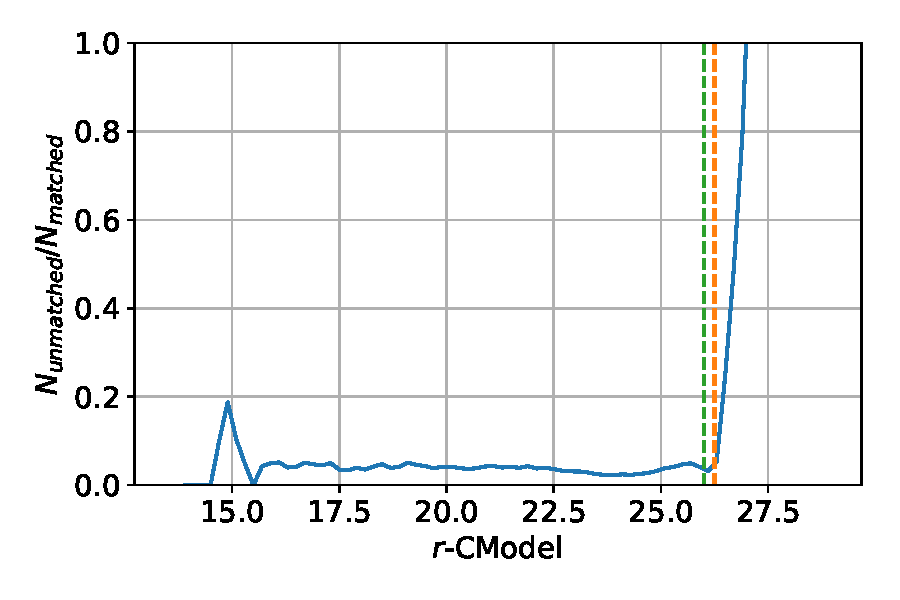
\includegraphics[width=0.9\columnwidth]{unmatched_fraction_magnitude.pdf}
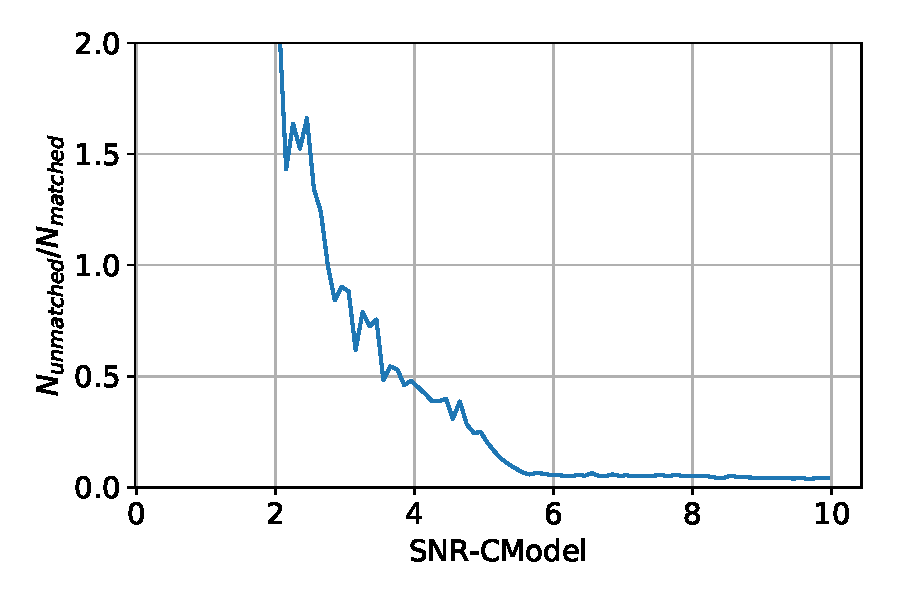
\includegraphics[width=0.9\columnwidth]{unmatched_fraction_SNR.pdf}
\caption{Top: Ratio of unmatched to matched primary detected sources after selection cuts as a function of magnitude. The dashed vertical lines show the median depth for the dithered (orange) and undithered (green) fields. Bottom: Ratio of unmatched to matched primary detected sources after selection cuts as a function of SNR.}
\label{fig:snr_mag_selection}
\end{figure}

\subsection{Star/galaxy classification}

For weak lensing and clustering analyses, it is important to have a pure galaxy sample, and a good control over the fraction of stars that are classified as galaxies. Our pipeline includes the variable \texttt{base\_ClassificationExtendedness\_value} (see~\citet{2018PASJ...70S...5B} for more details) , which we will refer to as extendedness, which can be used as a proxy to separate stars from galaxies as showed by~\citet{2018PASJ...70S..25M} and~\citet{2018PASJ...70S...5B}. In this work we say that an object has been classified as a galaxy if extendedness=1, and that the object has been classified as a star if extendedness=0. Now we are going to check how extendedness performs as star/galaxy classifier in DC1. In order to do so, we use the \textit{clean sample} with $16 \leq r \leq 26$ in the dithered field, although we find similar results using the undithered field, and match it to our input catalog. After that, we count the number of objects matched to stars that have been classified as stars, as a function of magnitude, and divide this number by the total number of objects matched to stars (which we will mark as Star $\rightarrow$ Star). We do the same with the number of objects matched to stars that have been classified as galaxies, and divide this number by the total number of objects matched to galaxies (Star $\rightarrow$ Galaxy); the number of objects matched to galaxies that have been classified as galaxies divided by the total number of objects matched to galaxies (Galaxy $\rightarrow$ Galaxy); and finally, the total number of objects matched to galaxies that have been classified as stars, divided by the total number of objects matched to stars (Galaxy $\rightarrow$ Star). This way, we know the total stellar (or galaxy) contamination as a function of measured magnitude. The results are depicted in \figref{star_galaxy_separation}. We see that at the brighter end ($r \leq 17$), there are a lot of stars that get classified as galaxies, this is due to two reasons: First, the ratio number of stars to number of galaxies at those magnitudes is larger than at fainter magnitudes, since stars and galaxies have different magnitude distributions. Second, problems related to saturation make difficult to use extendedness as a proxy for distinguishing stars and galaxies. On the other hand, we see that at the fainter end ($r \approx 26$), the purity of the galaxy sample using the extendedness classifier starts to decrease, getting as low as 90\% for the last bin in our analysis, and an overall $f_{star}=2.8\%$ stellar contamination in the \textit{clean sample} after using extendedness=1. This number gets reduced to $f_{star}=1.4\%$ if we only consider galaxies with $r < 25.5$, and $f_{star}=0.7\%$ for $r < 25$. Note that these number are larger than those in~\citet{2018PASJ...70S..25M}. This is mostly due to the fact that our PSF is larger, making the extendedness classifier perform a little bit worse, and that we do not include any cuts in resolution. However, this level of stellar contamination is acceptable for the purposes in this work.

\begin{figure}
\centering
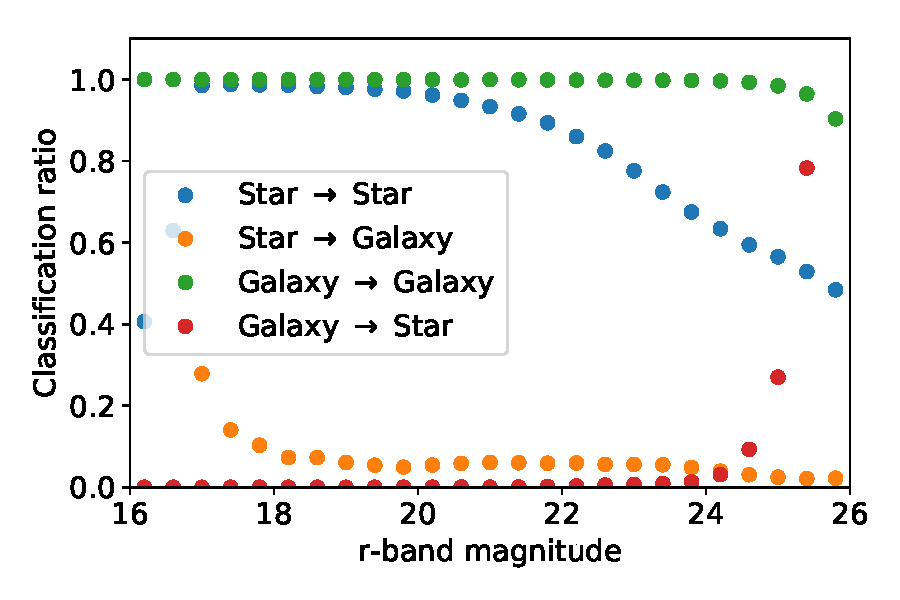
\includegraphics[width=0.9\columnwidth]{stellar_contamination}
\caption{Fraction of objects correctly classified as stars (blue) or galaxies (green), and fraction of objects misclassified as stars (red) or galaxies (orange) as a function of magnitude in the dithered field. The results are equivalent in the undithered case.}
\label{fig:star_galaxy_separation}
\end{figure}
\subsection{Depth maps and footprint masking}
\label{sec:masking}

In order to estimate the depth in the coadd catalogs we generate a flat-sky map, with resolution of $1.74$ arcminutes, containing the detected primary sources in the \textit{clean sample} from the previous subsection. This resolution ensures having an accurate estimate of the power-spectra up to $\ell \sim 6000$, where the power-spectra will be mostly dominated by shot-noise. Then, for each pixel, we compute the median SNR of the objects in that pixel as a function of the magnitude and use the magnitude at which SNR is closest to 5.

These maps are shown in \figref{depth_maps}. We can see that the dithered simulation is indeed very uniform ($> 50\%$ of its footprint lie in the same exact depth bin) showing the success of the dither strategy. However, we can see that in the undithered simulation, as expected, there are zones with a higher depth (the overlap of the pointing positions) and a reduced median depth.
\begin{figure}
\centering
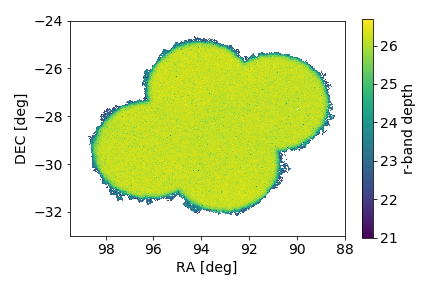
\includegraphics[width=0.9\columnwidth]{dithered_depth.png}
%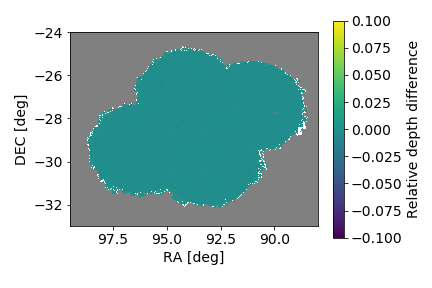
\includegraphics[width=0.45\textwidth]{dithered_difference.png}
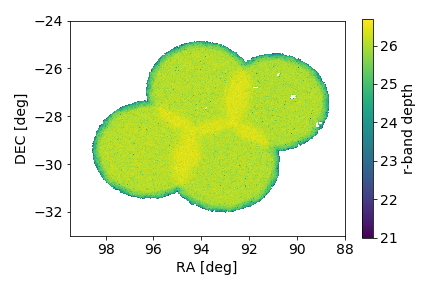
\includegraphics[width=0.9\columnwidth]{undithered_depth.png}
%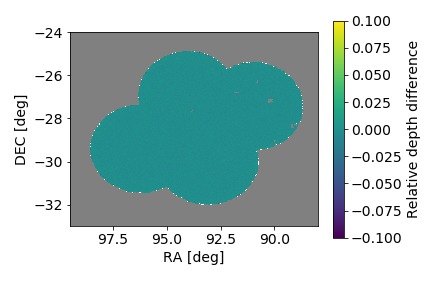
\includegraphics[width=0.45\textwidth]{undithered_difference.png}
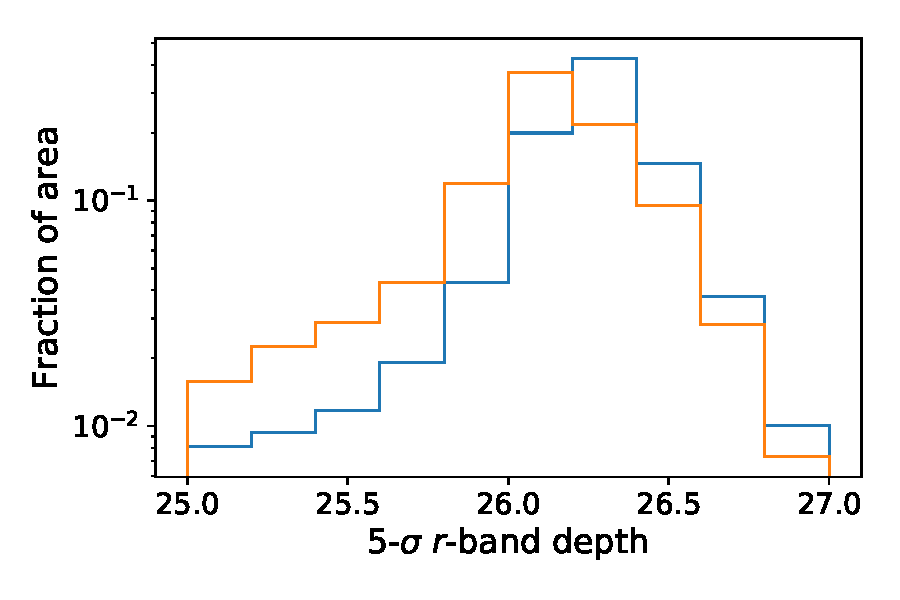
\includegraphics[width=0.9\columnwidth]{depth_comparison_1d.pdf}
\caption{5-$\sigma$ depth maps for the dithered (top) and undithered (middle) fields. There is an increased depth in the overlapping parts of the pointings in the undithered field but the median depth is lower. The maps have a resolution of $1.74$ arcmin. We also show the 1D distribution of depth (bottom) for both fields for easier comparison.}
\label{fig:depth_maps}
\end{figure}

We also check the depth by checking the detection efficiency of stars as a function of magnitude. To do so, we use the stars in the input catalog and select those that lie within the simulated footprint, after this, we match them using the spatial+magnitude technique described in previous sections. Finally, we compute the number of detected objects in the \textit{clean sample} matched to stars divided by the number of stars in the input catalog as a function of the magnitude of the matched object in the input catalog. The results can be seen in \figref{stellar_detection_efficiency}. We see that there is a high efficiency $> 80\%$ up to $r \approx 25.8$. 
\begin{figure}
\centering
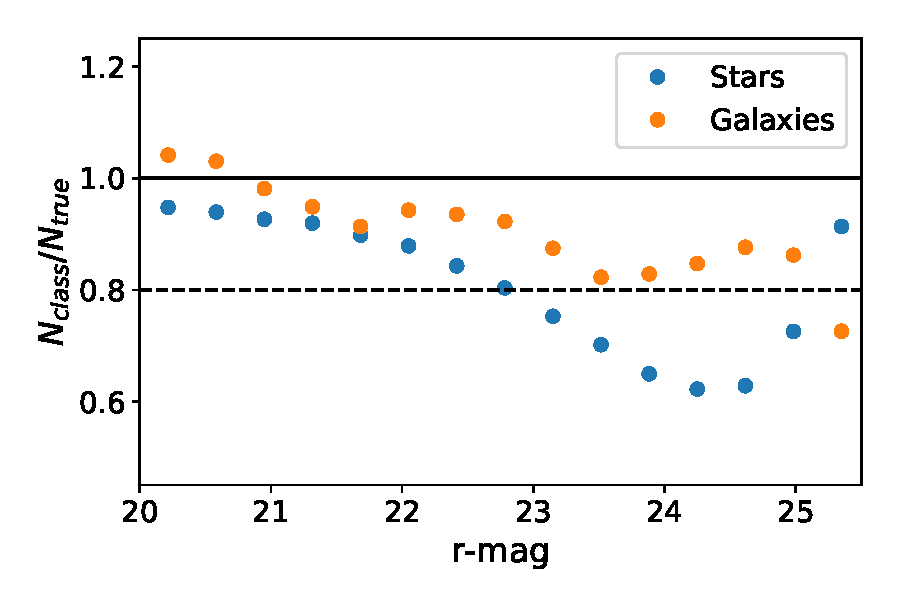
\includegraphics[width=0.9\columnwidth]{stellar_detection_efficiency.pdf}
\caption{Ratio of number of detected objects matched to stars in the \textit{clean sample} and number of stars in the input catalog as a function of magnitude for the dithered (blue) and undithered (orange).}
\label{fig:stellar_detection_efficiency}
\end{figure}

Given the results in the two previous subsections and this subsection, we decide to use only the galaxies that lie in pixels with limiting magnitude $r \geq 25.5$ and select those objects with magnitude $17 \leq r \leq 25.5$. This cut ensures high completeness ($>85\%$), as well as that we eliminate most of the artifacts in the sample, and that we have a low stellar contamination ($f_{star} \approx 1.4\%$). After these cuts and selecting objects with extendedness=1, we obtain 5.1 and 4.8 million objects for the dithered and undithered fields respectively.

\subsection{Bright object masking}

Bright objects produce significant effects in the image that affect the detection and measurement of neighboring objects. Some examples of these effects include saturation, large diffraction spikes, obscuration of neighboring sources, etc. Thus, masking a region around these sources creates a more complicated footprint but greatly simplifies the analysis of systematic effects. In order to avoid possible biases by masking bright galaxies we will only analyze the impact of bright stars in the nearby detected objects. In the following, when we refer to bright object masking we are actually referring to bright star masking.

In order to evaluate the effects, we follow the procedure described in \citet{2018PASJ...70S...7C}, modifying it accordingly to the availability of our input data. Using the position of stars in the input catalog, that lie within the considered footprint, and with input magnitudes in the range $m_{1} < r < m_{2}$ we count all primary detected objects (avoiding any other selection cuts) in a given radius $\theta$, and compute the median of the set, $N_{neighbors}$. We repeat this for different radii and magnitude ranges. Finally, we repeat this process for all stars in the input catalog in the footprint and compute $N_{neighbors, tot}$ and compute the ratio $y = N_{neighbors}/N_{neighbors, tot}$. We fit this ratio to an error function:
\begin{equation}
y_{model} = \mathrm{Erf}\left({\theta/\theta_{mask}}\right)
\end{equation}
This fit is performed for the first three bins in stellar magnitude that we consider, $r < 14$, $14 < r < 16$, and $16 < r < 18$. We ignore the points with $\theta < 10$ arcsec for the fit. Following \citet{2018PASJ...70S...7C} we use the point where the density reaches 95\% as masking radius, i.e., $r_{mask,fit} = \mathrm{Erf}^{-1}(0.95) \theta_{mask}$. After this, we compare to equation (1) in \citet{2018PASJ...70S..25M}:
\begin{equation}
r_{mask,HSC} = 200\times 10^{0.25(7-m_{B*})} + 12 \times 10^{0.05(16-m_{B*})} 
\end{equation}
Where $m_{B*}$ is the magnitude of the bright star to mask. Note that this prescription is specific for HSC. However, the LSST instrument and observing conditions are different. This is why we decided to rescale $r_{mask,HSC}$ by the ratio of mean seeing in LSST and HSC.
\begin{equation}
r_{mask,LSST} = r_{mask,HSC} \frac{1.04\arcsec}{0.58\arcsec}
\end{equation}
Where 1.04\arcsec is the mean seeing in DC1, and 0.58\arcsec is the mean seeing reported in~\citet{2018PASJ...70S..25M}. We obtain the results depicted in \figref{bright_object_masking}. We see that the error function describes well the behavior for $N_{neighbors}/N_{neighbors,tot}$. We also see that the masking radius, $r_{mask,LSST}$, using the rescaled prescription set by \citet{2018PASJ...70S..25M} is a pretty good approximation for our data. In particular, we find that the ratio $r_{mask,fit}/r_{mask,LSST} \approx 1.14$. This 14\% disagreement can be related to the fact that we chose a very simple rescaling based on the mean seeing and due to our simplistic PSF model. As a result, we decide to use $r_{mask, DC1} = 1.14 r_{mask, LSST}$ around stars in the input catalog with $r < 16$, since this is the saturation limit for LSST. We generate a high-resolution mask using flat-sky maps of $\approx 12.9 \arcsec$ resolution, then we downsample this map to a resolution of $\approx 2$ arcmin and eliminate objects that lie within pixels that have more than 50\% of their area masked. This results into a total area loss of $\approx 27.5\%$ of our footprint, which can be seen in \figref{bo_mask}. After these cuts we keep 3.74 million in the dithered field and 3.51 million in the undithered field.
\begin{figure}
\centering
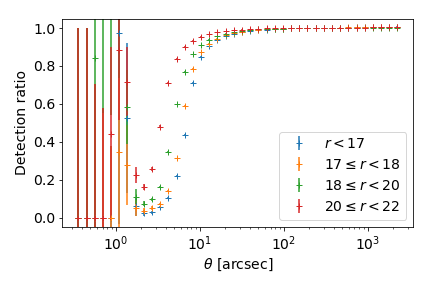
\includegraphics[width=0.9\columnwidth]{bright_object_masking}
\caption{Ratio of the median number of primary detected objects neighboring a star in a certain magnitude range in the input catalog to the median number of objects detected any star in the input catalog, as a function of the distance to the star $\theta$. Different symbols and colors represent different magnitude ranges for the stars in the input catalog considered. The shadowed regions represent the best fit masking radius, $r_{mask,fit}$ with their uncertainties and the vertical lines correspond to $r_{mask,LSST}$ evaluated at the mean magnitude in each bin.}
\label{fig:bright_object_masking}
\end{figure}
\begin{figure}
\centering
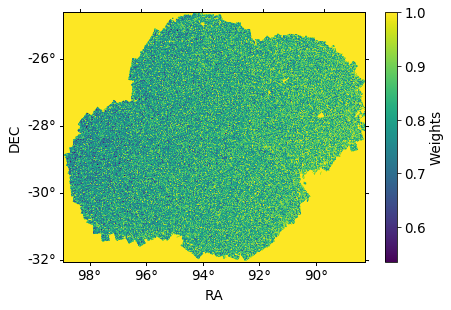
\includegraphics[width=0.9\columnwidth]{bo_mask}
\caption{Bright object (bright star) mask. This map shows with 1 (yellow) the pixels that we will consider for our analysis, and with 0 (blue) the regions of the sky that will not be considered in our analysis using this mask. We use a high-resolution ($\approx 12.9 \arcsec$) map to mask around bright stars ($r < 16$) and then, we downsample the map to a lower resolution ($\approx 1.74 \arcmin$) and get rid of the pixels where the masked area by bright stars is higher than 50\% of the pixel. This bright}
\label{fig:bo_mask}
\end{figure} 
\subsection{Blending}
As previously mentioned, our output catalogs do not include any estimation of overlap between sources, or \textit{blendedness}~\citep{2018PASJ...70S...5B}. Highly-blended objects are more likely to have biased estimations of the centroid position, shape, and fluxes. This can lead to overall biases in the estimated photometric redshifts and cosmological parameters. Given that the mean seeing in DC1 is larger than in HSC, the impact of blended objects is likely to be larger. In the case of \citet{2018PASJ...70S..25M}, the cut in the blendedness parameter affects only 1\% of the objects; we expect this number to be larger in our case. Using specialized image simulations from~\citet{Sanchez19} with a seeing equal to the seeing in DC1 (1.04\arcsec), in $r$-band, we find that if we select objects with $r < 25.5$ and SNR $\geq 1$, the fraction of objects with blendedness $ >10^{-0.375}$ is $\approx 6.3\%$. If we raise the minimum SNR threshold to 6, this fraction is lowered to $\approx 2.6\%$. This means that our sample will have a fraction of these objects anywhere in the range (2.6\% - 6.3\%) but closer to 2.6\% since the fraction of objects with SNR $\leq 6$ is $\approx 0.3\%$. In any case, we do not expect that the inclusion of these objects in our two point measurements will affect the range of scales that we are going to consider in this work. In order to quantify this, a careful study of the impact of blending in clustering measurements is necessary but this is out of the scope of this work.

\section{Two-point clustering results}
\label{sec:results}

In this section, we analyze the two point clustering statistics for both the dithered and undithered catalogs in harmonic space and check the consistency between the input and measured observables. We also analyze the impact of different observing conditions in two-point statistics. 

In order to measure the angular power spectrum, we use \texttt{NaMaster}\footnote{\url{https://github.com/LSSTDESC/NaMaster}}~\citep{2019MNRAS.484.4127A}. \texttt{NaMaster} allows us to compute the cross-power-spectra of spin-0 and spin-2 maps, with an arbitrary mask and number of contaminants using the pseudo-$C_{\ell}$ formalism~\citep{1973ApJ...185..413P,2002ApJ...567....2H,2017MNRAS.465.1847E}. In this case, we focus on the angular power spectrum of the density contrast map, $\delta$. Given the lack of photometric redshift measurements in our data, we decided to analyze full \textit{final sample}. We check the range $0 < \ell < 6000$ in bandpowers of $\Delta \ell = 352$ and ignore the first bin due to lack of sensitivity at that range of scales ($\ell=178 \approx 2$ degrees). The choice of $\Delta \ell$ was done so the resulting covariance matrix is close to diagonal although we opted to make 4 times more bins that the optimal $\Delta \ell_{opt} = 1/f_{sky}$, with $f_{sky}$ being the fraction in the footprint. However, we are going to only consider multipoles such that $\ell \geq 1/f_{sky} \approx 1574$. We estimate the Gaussian covariance with \texttt{NaMaster} obtaining the results in~\figref{gaussian_cov}. Given that we are focused on demonstrating the ability to perform end-to-end analysis, this Gaussian covariance will be enough for our purposes. However, careful computation of the non-Gaussian contributions to the covariance should be performed in the case of performing any cosmological analyses given the size of our footprint.

\begin{figure}
\centering
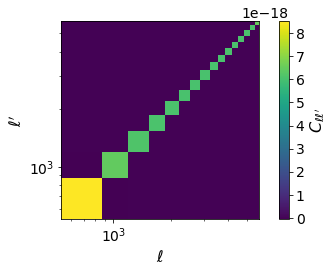
\includegraphics[width=0.9\columnwidth]{Gaussian_covariance}
\caption{Estimated Gaussian covariance using \texttt{NaMaster} in the range of scales considered in our analysis.}
\label{fig:gaussian_cov}
\end{figure}

The DC1 simulations also allow us to study the effect of different observational effects in the two-point clustering statistics and how the dithering strategies work to mitigate these effects. We are going to consider the following effects:

\begin{itemize}
\item Extinction: The CatSim catalog provides the value for the magnitudes corrected for extinction using the map from \citet{1998ApJ...500..525S}, which we refer to as the SFD map.
\item Stellar contamination: In this case, we build a flat-sky map with all stars in the input catalog.
\item Sky-background/Sky-brightness: We use the observed background level in each exposure and assign that value to the pixels in the flat-sky map that lie within that exposure. After this we calculate the mean value in each pixel to build the map with the same resolution as the mask ($\approx 2$ arcmin) which we deproject~\citep{2019MNRAS.484.4127A}. 
\item Sky-noise: We use the observed noise background level in each exposure and proceed as in the previous case to build a map.
\item Seeing: We proceed as before and use the observed seeing in each exposure and build a map.
\item Number of visits: We count the number of exposures overlapping with each pixel of our flat-sky maps.
\end{itemize}
These maps are shown in \figref{systematic_maps} and \figref{systematic_maps_ud}. We see that the spatial distribution of the different observing conditions are very different between the two simulations, even though the ranges in each of the observing conditions are very similar. 

\begin{figure*}
\centering
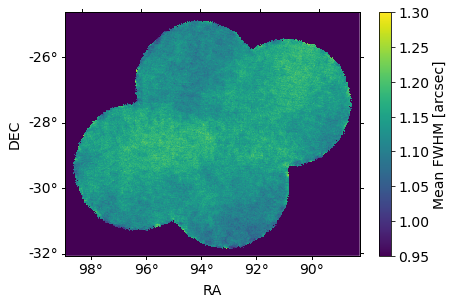
\includegraphics[width=0.45\textwidth]{mean_fwhm.png}
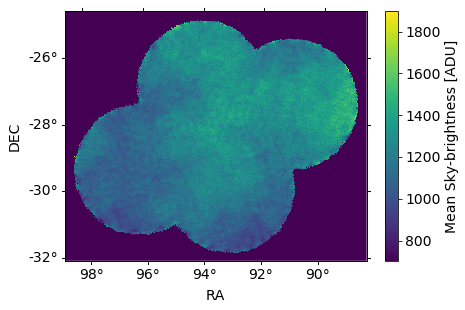
\includegraphics[width=0.45\textwidth]{mean_sky.png}
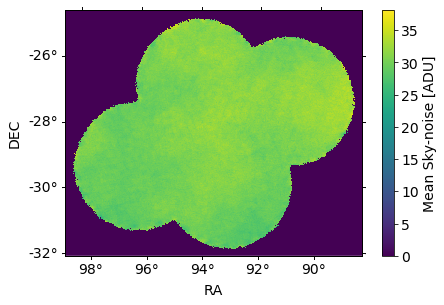
\includegraphics[width=0.45\textwidth]{mean_skynoise.png}
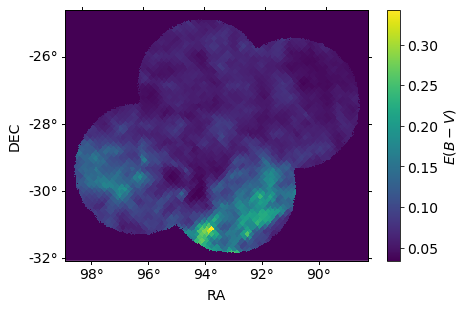
\includegraphics[width=0.45\textwidth]{extinction.png}
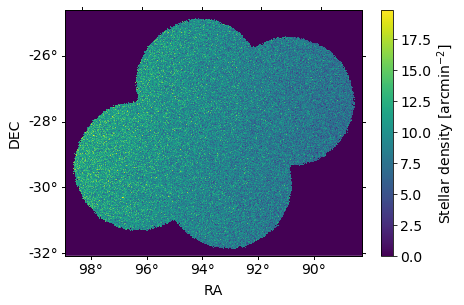
\includegraphics[width=0.45\textwidth]{stellar_density.png}
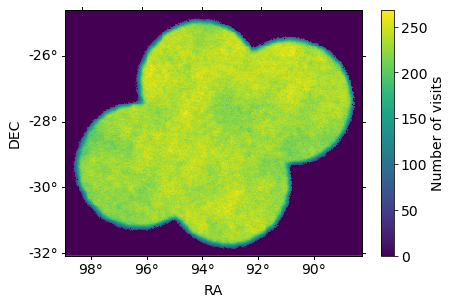
\includegraphics[width=0.45\textwidth]{nvisits.png}
\caption{Maps showing the different foregrounds considered in our analysis of the dithered field. From top left to bottom right: Mean PSF FWHM, mean sky-brightness, mean sky-noise, mean extinction, stellar density and number of visits in each pixel in the flat-sky maps with the same resolution as the depth maps in \figref{depth_maps}. We only show their values in the regions where the 5-$\sigma$ $r$-band depth is larger than 25.5.}
\label{fig:systematic_maps}
\end{figure*}

\begin{figure*}
\centering
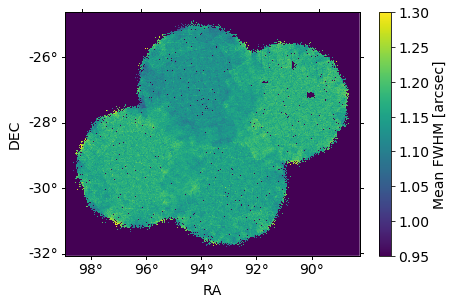
\includegraphics[width=0.45\textwidth]{ud_mean_fwhm.png}
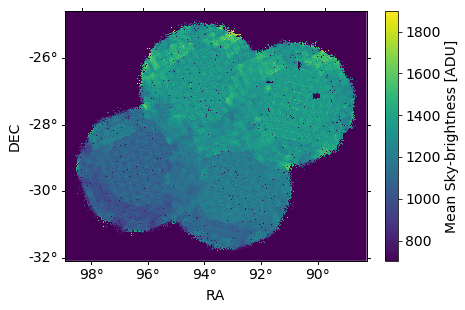
\includegraphics[width=0.45\textwidth]{ud_mean_sky.png}
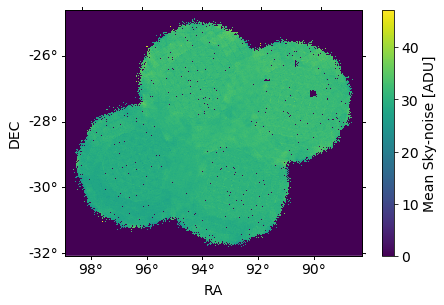
\includegraphics[width=0.45\textwidth]{ud_mean_skynoise.png}
%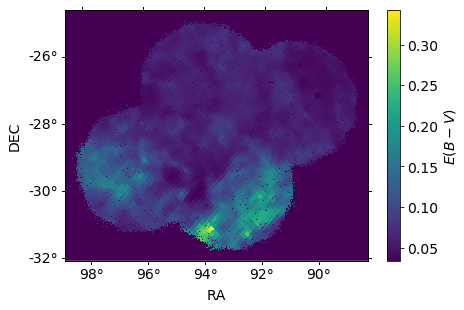
\includegraphics[width=0.45\textwidth]{ud_extinction.png}
%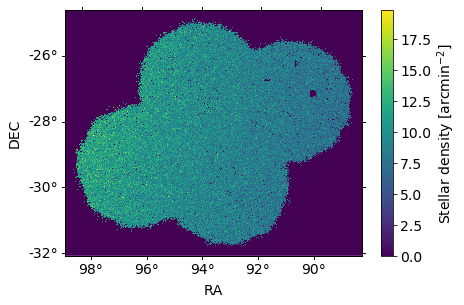
\includegraphics[width=0.45\textwidth]{ud_stellar_density.png}
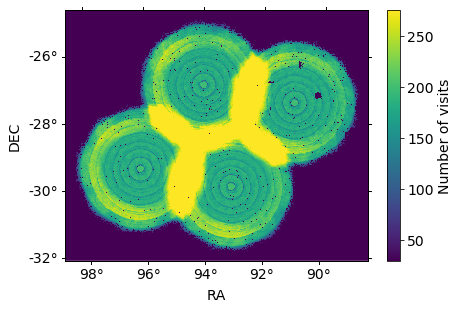
\includegraphics[width=0.45\textwidth]{ud_nvisits.png}
\caption{Same as \figref{systematic_maps} for the undithered dataset. From top left to bottom right: Mean PSF FWHM, mean sky brightness, mean sky noise and number of visits. Note that we use the same extinction and stellar density maps changing the geometry of the mask.}
\label{fig:systematic_maps_ud}
\end{figure*}

We use the mode deprojection from \texttt{NaMaster}~\citep{2019MNRAS.484.4127A} to correct for the potential contamination of the maps described above. Mode deprojection, assumes that there is a linear dependency between the observed number density of galaxies and the contaminants. We checked that this is a good approximation for the different observing conditions. In addition, we compute the theoretical prediction for the power-spectra with \texttt{CCL}:
\begin{equation}
C_{\ell}^{\rm TH} = \frac{2}{\pi}\int{dz} \left(\frac{dn(z)}{dz}\right)^{2} b^{2}(z) \int{dk k^{2} P(k,z)j^{2}_{\ell}(kr(z))}
\end{equation}
where $P(k,z)$ is the power spectrum, $b(z)$ is the bias and $\frac{dn}{dz}$ is the number density as a function of redshift. We use the Millenium cosmological parameters~\citep{2005Nature.435.629S} ($\Omega_{m}=0.25$,$\Omega_{b}=0.045$,$\Omega_{\Lambda}=0.75$, $n=1$, $\sigma_{8}=0.9$, $h=0.73$), and the $dn/dz$ built by using the true redshifts in galaxies matched in the input catalog. We use a constant value for the bias $b$ that we fit by minimizing the following $\chi^{2}$:
\begin{equation}
\chi^{2}=\sum_{\ell,\ell^{\prime}}\left(C_{\ell}^{data}-b^{2} C_{\ell}^{th}\right)\mathcal{C}_{\ell,\ell^{\prime}}^{-1}\left(C_{\ell}^{data}-b^{2} C_{\ell}^{th}\right)
\end{equation}
By doing so we obtain $b = 0.35 ^{+ 0.09}_{- 0.13}$ (considering only $\ell \geq 1574$). We validated these results by comparing with the bias obtained using measurements in real space (two point correlation function), where we obtain results compatible within 1-$\sigma$, even at larger scales than those considered for our analysis. In \figref{power_spectra} we see that the measured power-spectra for both datasets follows the theoretical prediction within errors, even for multipoles $\ell$ smaller than those considered in our fit. We see that the constant linear bias model is a very good approximation in this case with $\chi^{2}=0.44$. However, this is not guaranteed when using smaller redshift slices in real data. This low value for $\chi^{2}$ manifests the need to take into account other contributions to the covariance, such as the super-sample covariance that we ignored in our analysis. In addition, we see that the overall impact of the systematics is smaller than 20\% of the statistical uncertainty in the range of scales considered. We also see that the observing conditions similarly affect both dithered and undithered simulations. Surprisingly, the undithered field seems to be slightly less affected by the observing conditions than the dithered field, especially at larger scales. However, the difference is not statistically significant. This is a consequence of several factors, including the conservative cuts that we impose on our data to ensure well-behaved clustering statistics; that we only deproject using the mean value for the different observing conditions; and the lack of effects, such as vignetting, present in real images. For example, vignetting would affect the number of detected objects close to the edges of the focal plane in the undithered simulation, reducing the uniformity of the survey. However, this effect would be uniform across the footprint in the dithered case. In addition to this, if we decided to push further our data by going deeper, the systematic lack of uniformity of the undithered field would start to play a large role in the impact of the foregrounds. We can also see that, in the $\ell$ range that we consider for our analysis, the presence of bright objects (BO) -- in particular bright stars -- is the dominant systematic effect. In the close neighborhood to bright objects ($r \leq 16$), our ability to detect faint sources diminishes. These faint sources are blended in the core or the tails of the brighter objects, resulting in a lower mean number of detected sources, as shown in \figref{bright_object_masking}. This showcases again the importance of considering the impact of blending in the low scale regime for LSST and should be carefully studied in future Data Challenges. The correction due to the presence of bright objects is comparable in both simulations.

\begin{figure}
\centering
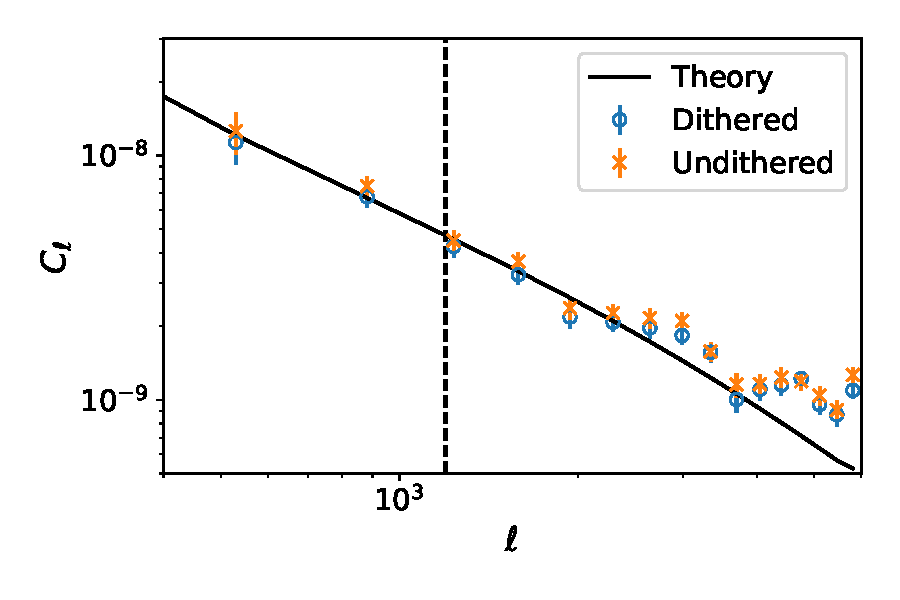
\includegraphics[width=0.9\columnwidth]{Cl_results_2019_comp}
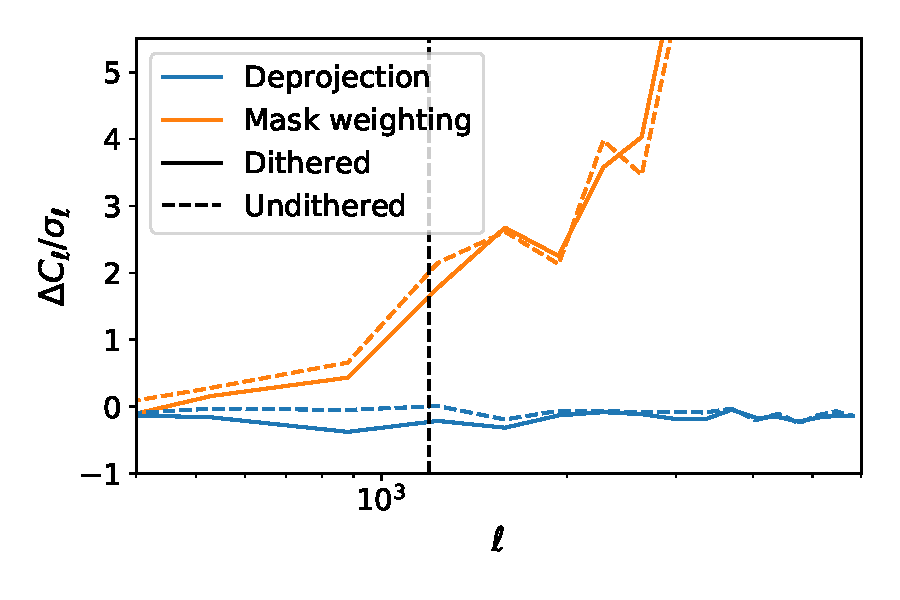
\includegraphics[width=0.9\columnwidth]{systematics_comp_abs}
\caption{{\bf Top panel:} Measured power spectra undithered (orange $\times$) and dithered (open blue circles) datasets with \texttt{NaMaster} corrected by systematics. The error bars are computed analytically via Gaussian approximation using \texttt{NaMaster}. The best-fit theoretical prediction is shown as the solid black line. The shadowed region corresponds to the 1-$\sigma$ confidence level for the galaxy bias. The vertical black dashed line corresponds to the minimum multipole considered for our analysis $\ell = 1/f_{sky}$. {\bf Bottom panel:} Size of the correction in the power-spectra, $\Delta C_{\ell}$, relative to their uncertainty, $\sigma_{\ell}$, due to deprojection (Dep.) of different observing conditions (blue), due to the presence of bright objects (BO, orange), and the total relative correction (green) for the dithered (solid lines) and undithered (broken lines) simulations.}
\label{fig:power_spectra}
\end{figure}

\section{Conclusions}
\label{sec:conclusions}

End-to-end simulations are powerful tools for testing the overall performance of any current and future cosmological experiments like the LSST~\citep{Overview}. They allow us to validate and improve on different parts involved in the data processing and analysis, as well as to model and improve our control of systematic uncertainties.

In this paper, we have presented a simulated (end-to-end) imaging dataset that resembles single-band, full-depth LSST data, for the first data challenge in the LSST DESC. We simulated images using state of the art tools (\textit{imSim}). We generated two different and complementary datasets, one with random dithers (\textit{dithered}) and the other with no dithers (\textit{undithered}). We processed these images with the LSST data management software stack and performed several quality assurance tests on its outputs. We checked that both the \textit{dithered} and \textit{undithered} are high-quality datasets and pass most of the LSST Science Requirements~\citep{LPM-17} and the DESC Science Requirements~\citep{2018arXiv180901669T} allowed by our design choices.

We studied different ways to relate the output catalogs to the inputs. In particular, we studied two different matching strategies. The first, using information about positions only and a second strategy involving positions and magnitudes. We showed that, for clustering analyses, adding information about magnitudes results in a lower incidence of spurious matches. The usage of matching strategies helped us define a clean sample suitable for clustering analyses. However, these matching techniques are likely not suitable for studies on blending or scales smaller than those considered in this work, since they do not include information about undetected sources present in blends. Therefore, an important research topic for these kinds of end-to-end simulations is to find efficient strategies to relate inputs and outputs.

We estimated the depth of our simulated catalogs and checked the impact of the presence of bright objects in the detected number density. After this, we selected a high-completeness sample to perform clustering analysis in harmonic space and used \texttt{NaMaster} to deproject the impact of simulated foregrounds. We find that in the case where we do not split the sample into different redshift bins, a constant linear bias well describes our data for the dithered and undithered simulations. The results of this analysis indicate that the simulated foregrounds have a low impact ($\approx 5\%$ of the statistical uncertainty) at the scales considered for our study ($1574 \leq \ell < 6000$) in both datasets. However, in this scale-range, the presence of bright objects has a larger impact on the power-spectra, $\approx 20\%$ of the statistical uncertainty, highlighting the impact of blending in LSST. 

Finally, we have been able to perform an end-to-end test of our processing and analysis pipelines, which will allow us to better prepare to exploit future LSST data.

The methodology presented in this work will serve as the basis for future DESC data challenges, where we aim to perform multi-band studies in a larger area, analyze complementary image generation strategies (\texttt{PhoSim}), and increase the complexity of the foregrounds included.

% ----------------------------------------------------------------------

\subsection*{Acknowledgments}

This research used resources of the National Energy Research Scientific Computing Center, a DOE Office of Science User Facility supported by the Office of Science of the U.S. Department of Energy under Contract No. DE-AC02-05CH11231. We acknowledge the use of \texttt{Pandas, Dask, SciPy, Matplotlib, Jupyter, CCL, NaMaster, Healpy, and scikit-learn} as well as the LSST software stack.

The work of JC, RD, SD, TG, AJ, HK, PJM and BVK was supported by the U.S. Department of Energy under contract number DE-AC02-76SF00515. 
The work of RM was supported by the US Department of Energy Cosmic Frontier program, grant DE-SC0010118.

%
The DESC acknowledges ongoing support from the Institut National de Physique Nucl\'eaire et de Physique des Particules in France; the Science \& Technology Facilities Council in the United Kingdom; and the Department of Energy, the National Science Foundation, and the LSST Corporation in the United States.  DESC uses resources of the IN2P3 Computing Center (CC-IN2P3--Lyon/Villeurbanne - France) funded by the Centre National de la Recherche Scientifique; the National Energy Research Scientific Computing Center, a DOE Office of Science User Facility supported by the Office of Science of the U.S.\ Department of Energy under Contract No.\ DE-AC02-05CH11231; STFC DiRAC HPC Facilities, funded by UK BIS National E-infrastructure capital grants; and the UK particle physics grid, supported by the GridPP Collaboration.  This work was performed in part under DOE Contract DE-AC02-76SF00515.
This manuscript has been authored by Fermi Research Alliance, LLC under Contract No. DE-AC02-07CH11359 with the U.S. Department of Energy, Office of Science, Office of High Energy Physics.

% 


\bibliography{lsstdesc,main}

\end{document}


% ======================================================================
%
